\documentclass[11pt,a4paper]{report}

% Aberstwyth MMP Project Report Template for LaTeX
%
% Authors: Neil Taylor (nst@aber.ac.uk) and Dr. Hannah Dee (hmd1@aber.ac.uk) 
%
% This has been adapted from the Leeds Thesis template and the 
% Group Project template for Computer Science in Aberystywth University.
% 
% All comments and suggestions welcome.
%
% Template designed to be used with pdflatex: it may need alteration to
% run with a different LaTeX engine.
%
% Note - this is offered as a starting point for your work. You are not 
% required to use this template and can choose to create your own document 
% without it.

% This template is suitable for students with an engineering-style project, 
% which will be most students in the department. If your project is a research-oriented 
% project, look at the alternative template.

% To build document on the unix command line, run four commands:
 
% pdflatex mmp-report
% bibtex mmp-report
% pdflatex mmp-report
% pdflatex mmp-report

% you will end up with mmp-report.pdf. Before submitting, add your user ID as a prefix, 
% e.g. abc01-mmp-report.pdf 
\usepackage{StylesAndReferences/mmp-report}

% the following packages are used for citations - You only need to include one. 
%
% Use the cite package if you are using the numeric style (e.g. IEEEannot). 
% Use the natbib package if you are using the author-date style (e.g. authordate2annot). 
% Only use one of these and comment out or remove the other one. 
\usepackage{cite}
%\usepackage{natbib}

%%%% Title and Section Colours %%%%
% Modify these values to change the colours used for title, sections and subsections.
% Each value is a range of 0-255 in RGB colourspace.
% Idea courtesy of discussion at 
% https://www.overleaf.com/learn/latex/Using_colours_in_LaTeX
% and
% https://tex.stackexchange.com/questions/75667/change-colour-on-chapter-section-headings-lyx
% 
% If you prefer to have black headers, then comment out the following lines
\definecolor{mmpTitle}{RGB}{10, 85, 145}
\definecolor{mmpSection}{RGB}{10,85,155}
\definecolor{mmpSubsection}{RGB}{79,129,189}

\chapterfont{\color{mmpTitle}}  % sets colour of chapters
\sectionfont{\color{mmpSection}}  % sets colour of sections 
\subsectionfont{\color{mmpSubsection}} % sets colour subsections
\subsubsectionfont{\color{mmpSubsection}} % sets colour subsections

%%%% end of Title and Section Colours %%%%


%%%% Report Type %%%%
%% comment/uncomment depending on the type of report you want to generate
\reporttype{Engineering}
%\reporttype{Research}
%%%% end of Report Type %%%%


\begin{document}

%TC:ignore

% all of the include directives below refer to tex files
% so %TC:ignore 

\title{Development of a map-based web application showcasing the Dyfi Wildlife Centre}

% Your name
\author{Michael Male}

% Your email 
\authoremail{mim39@aber.ac.uk}

\degreeschemecode{G40F} %e.g. G400 
\degreeschemetitle{Computer Science (includes Foundation Year)} % e.g. Computer Science
\degreetype{BSc}

\modulecode{CS39440} % i.e. CS39440, CC39440, CS39620
\moduletitle{Major Project} % i.e. Major Project or Minor Project

\date{10th May 2020} % i.e. the date of the current version of your report

\status{Draft} % Use draft until you create the release version. Then, change this to Release.
\version{0.8}

% The title and name of your supervisor.
\supervisor{Dr Edel Sherratt} 

%The email for your supervisor. 
\supervisoremail{eds@aber.ac.uk}

\maketitle

%TC:endignore
 includes cover.tex - to change the content,
% edit the tex file

\pagenumbering{roman}

% This is the front page
%TC:ignore 

\title{Development of a map-based web application showcasing the Dyfi Wildlife Centre}

% Your name
\author{Michael Male}

% Your email 
\authoremail{mim39@aber.ac.uk}

\degreeschemecode{G40F} %e.g. G400 
\degreeschemetitle{Computer Science (includes Foundation Year)} % e.g. Computer Science
\degreetype{BSc}

\modulecode{CS39440} % i.e. CS39440, CC39440, CS39620
\moduletitle{Major Project} % i.e. Major Project or Minor Project

\date{10th May 2020} % i.e. the date of the current version of your report

\status{Draft} % Use draft until you create the release version. Then, change this to Release.
\version{0.8}

% The title and name of your supervisor.
\supervisor{Dr Edel Sherratt} 

%The email for your supervisor. 
\supervisoremail{eds@aber.ac.uk}

\maketitle

%TC:endignore
                        

% Set up page numbering
\pagestyle{empty}

% declarations of originality 
\thispagestyle{empty}

%TC:ignore

%%%
%%% You must sign the declaration of originality. 
%%%
%%% You are submitting this electronically. Therefore, to sign, you 
%%% type your name and date to replace the .... characters. 
%%%
\section*{\centering Declaration of originality}

I confirm that:

\begin{itemize}
\item{This submission is my own work, except where 
clearly indicated.}

\item{I understand that there are severe penalties for Unacceptable Academic Practice, which can lead to loss of marks or even the withholding of a degree.}
 
\item{I have read the regulations on Unacceptable Academic Practice from the University's Academic Registry (AR) and the relevant sections of the current Student Handbook of the Department of Computer Science.}
 
\item{In submitting this work I understand and agree to abide by the University's regulations governing these issues.}
\end{itemize}

\vspace{2em}
Name Michael Male  \\

\vspace{1em}
Date 10/05/2020 \\

%%% 
%%% We would like to make a selection of final reports available to students that take 
%%% this module in future years. To enable us to do this, we require your consent. You 
%%% are not required that you do this, but if you do give your consent, then we will have 
%%% the option to select yours as one of a number of reports as examples for other 
%%% students. If you would like to give your consent, then please include the following 
%%% text and type your name and date to replace the .... characters. 
%%% 
%%% If you do not wish to give your consent, please remove this from your report. 
%%%
\vspace{1em}
\section*{\centering Consent to share this work}

By including my name below, I hereby agree to this project's report and technical work being made available to other students and academic staff of the Aberystwyth Computer Science Department.  

\vspace{2em}
Name Michael Male  \\

\vspace{1em}
Date 10/05/2020 \\

%TC:endignore

               

\thispagestyle{empty}

%TC:ignore

\section*{\centering Acknowledgements}


I am grateful to Mr Emyr Evans and Mr Thomas Faulkner of the Montgomeryshire Wildlife Trust for their support in the development of this project, and hope that the final product is useful to them.

I'd like to thank my supervisor, Dr Edel Sherratt, for her help, support and encouragement during all stages of this project, as well as Mr Richard Shipman, who provided useful feedback in the mid-project demonstration that ensured the project was kept afloat.

%TC:endignore % Acknowledgements

\thispagestyle{empty}

%TC:ignore

\section*{\centering Abstract}

The Dyfi Wildlife Centre is a visitor centre run by the Montgomeryshire Wildlife Trust. It is situated on the Cors Dyfi Nature Reserve in Powys, Wales. The Trust had approached the University, with a request for a solution to assist in showcasing the reserve's work, and its place as an osprey conservation, engagement, and research project. They had procured an 86-inch touchscreen monitor, in the hopes of presenting an application that aids in achieving the aforementioned goal.

The software created in this project takes the form of a map-based web application. The frontend makes use of the Google Maps for JavaScript API, as well as HTML, CSS and Thymeleaf, to show visitors a map of the centre and its surroundings. The map has various markers, and filters, that can be clicked on, showing further information about the point of interest. This is backed up by a RESTful API backend, creating using the Spring Framework, a model-view-controller framework with for Java Enterprise Edition. An administration panel was also developed, involving authentication, and allowing the authenticated user to add, edit, and delete points of interest. Data was stored in a PostgreSQL relational database.

Planning and development of this project took the form of an agile approach, with ideas from both Kanban and Extreme Programming used and adapted to fit a single-developer project. A meeting with the customer took place prior to development, and user stories and prioritisation of tasks had branched out from that meeting. The concept of test-driven development was a driving force for the development of this project, with various testing suites including JUnit, HTMLUnit and Selenium utilised when creating test cases. A key part of this project was ensuring that the customer was kept up-to-date, and supplementary documentation was created for this project that provided a brief overview of the required setup and how to use the web app.



%TC:endignore                 % Abstract

\pagenumbering{roman}
\pagestyle{fancy}
\fancyhead{}
\fancyfoot[C]{\thepage}
\renewcommand{\headrulewidth}{0 pt}
\renewcommand{\chaptermark}[1]{\markboth{#1}{}}

\tableofcontents   
\newpage
\listoffigures % comment out this line if you don't have any figures / graphics
\newpage 
\listoftables % comment out this line if you don't have any tables
\newpage

% Set up page numbering
\pagenumbering{arabic}

\setchapterheaderfooter

%TC:endignore

% include the chapters
\chapter{Background \& Objectives}

\section{Background}

A number of key considerations were taken into place during the background planning stages of this project.

An initial meeting took place in February 2020 with the customer, the Montgomeryshire Wildlife Trust. The hardware implementation was discussed and it was understood that the customer would want to run the web application on an 86-inch touch screen monitor. They also expressed a preference for the web application to be run locally, and not published to a cloud service or the World Wide Web. Therefore, an important consideration of the project was enabling the web application to work using touch gestures, and use a responsive layout that would scale to a high resolution.

With the intention being that the application runs locally, therefore research had to be put into various technology stacks, and which web framework would work best for this kind of application. Research into this would have to take into account how much time needs to be allocated to performing spike work; ensuring a comprehensive understanding of the framework was achieved before work on the project began.

Another key consideration was the vendor for the maps API. A number of APIs were assessed for their usability as well as their licensing conditions.

In this section, the early investigative work into the project will be discussed, with an analysis of the steps taken to achieve a conclusion as to which technology stack to use. 

\subsection{Web Development Frameworks and Tools}

Early on in the project it was decided that the use of a comprehensive web framework would be beneficial to the usability and production quality of the web application. This was opposed to a simple HTML 5, CSS, and JavaScript stack. Whilst it was inevitable that portions of each language had to be used, a more robust framework provided specific advantages, such as a package manager and cleaner code.

Three primary web frameworks were assessed, through the use of research, prior reading, and spike work, these being the following:

\begin{itemize}
\item	A JavaScript-based framework, utilising the Node.js and Express backend frameworks and either Vue.js or React as the frontend.
\item	Django, a Python-based model-template-view framework.
\item	The Spring Framework, a Java-based model-view-controller framework.
\end{itemize}

Further research took place into the CSS frameworks, as well as an appropriate database management system. Discussion into these are expanded upon in their relevant sections.

\subsubsection{JavaScript Frameworks}

A full-stack JavaScript framework allowed for the benefit of the software being written in one programming language, which could reduce issues with the code's readability and maintenance. It would have also allowed for a single testing framework, such as Jest, a testing framework maintained by Facebook.
% Citation: https://link.springer.com/chapter/10.1007/978-1-4842-1260-8_9,https://jestjs.io/ 
The use of a runtime environment would be standard fare for a JavaScript framework, allowing sever-side scripting and dynamic web pages to be run outside of the usual web browser environment that JavaScript runs on. A popular JavaScript runtime is Node.js, which has been touted as a resource-efficient framework, a benefit for a project that is designed to run on a local computer.
% Citation: https://link.springer.com/article/10.1007/s00607-014-0394-9


Frontend frameworks were also looked at, with varying levels of spike work being put into them. React, a Facebook-maintained JavaScript library, and Vue.js, were both considered. The two frameworks are rather similar, such that they rely on sending data directly to the browser's Document Object Model, however Vue.js takes a declarative approach to HTML scripting, whilst React uses JSX, an HTML syntax extension to JavaScript.
% Citation: https://vuejs.org/v2/guide/comparison.html 


Ultimately, a lack of familiarity with JavaScript, as well as the relative complexities of the frameworks, proved to be a deciding factor in not going ahead with a JavaScript-driven application. During research, it was deemed that a large amount of time would have to be dedicated to following tutorials and learning JavaScript, and ECMAScript 6, from scratch, and this would have taken too much time and risked a less complete final product.

\subsubsection{Django}

Django is an open-source framework based on the Python programming language. Its creators set the framework's primary philosophies as a quick approach to development, a view to not repeating the design and execution of concepts, and loose coupling - in this context being that the framework layers shouldn't be able to interface with eachother unless necessary.
% Citation: https://docs.djangoproject.com/en/3.0/misc/design-philosophies/

Django utilises the object-oriented programming paradigm with Python, and utilises a model-template-view approach. In short, these are three distinct layers of a web application: the model consists of a data structure, the view consists of a representation of information on a web browser, and a controller allows access to this data with meaningful requests.
% Citation: https://ieeexplore.ieee.org/abstract/document/950428

Whilst Django appeared to be a good choice due to its highly cohesive pattern, testing of the setup proved to be difficult on occasion, with design patterns that were particularly unique to Django. Whilst Python is a language that is known to utilise concepts that are simple to understand for users with greater knowledge in other programming languages, utilisation of Python at this level required a higher level of expertise than was had at the time. It was decided that there would be a greater chance of success with the project if attention was placed more towards frameworks with a more familiar language, to avoid an inordinate amount of time being spent on the intricacies of specific programming languages and frameworks.
 
\subsubsection{Spring Framework}

The Spring Framework is an open-source framework, where its web application features are based upon Java Enterprise Edition, an enterprise specification of the Java programming language that has modules specifically tailored towards web services.
% Citation: https://www.oracle.com/java/technologies/java-ee-glance.html

Spring provides many of the benefits that Django also provides, and the two are often compared against eachother. Similar to Django, Spring utilises a model-view-controller framework, and relies upon high cohesion. As Spring uses Java, it takes advantage of the object-oriented programming paradigm, and it is standard for classes to be written in such a way that they follow this concept. Spring is optimised to work with the Thymeleaf template engine, that provides server-side scripting and an interface between the controller and view layers.
% Citation: https://www.thymeleaf.org/

Ultimately, a proficiency in Java from previous academic study and personal use made Spring an ideal choice for this project. Spring Boot, an addition to the platform that allows for automatic configuration of core dependencies, was also used, to reduce the amount of time spent studying elements of Spring that Spring Boot renders redundant. Spring also utilises Maven, a Java package manager, to provide a large number of dependencies; Spring Security was deemed a useful tool for an authentication layer, for example. An added benefit to Spring is its embedded Apache Tomcat server, that allows for the provision of an HTTP web server environment from opening the application, rather than having to take steps to deploy it into an existing web server environment.

\subsubsection{CSS frameworks}

It was decided in the planning stages of the project that it would be beneficial to use a CSS framework, rather than build a template with 'vanilla' implementations of HTML and CSS. CSS frameworks provide a large number of pre-built elements, many that are rather familiar to users, due to their prevalence in front-end web design. A review into three different CSS frameworks were performed.

Bootstrap, a framework initially developed for use with Twitter, provides elements that have been crafted with the User Experience at their forefront. It is used by a large variety of web applications and websites, with the developers claiming it is 'the world's most popular front-end component libary.' Whilst this would have been a good choice for a familiar user interface, the framework was assessed to have less customisability, which posed an issue with a unique implementation where the main aspect is a single-page application. Bootstrap is also intended to be mobile-first, a feature that is not required, as the application is designed to run on a desktop computer.
%Citation: http://51.255.68.3:8011/143.95.72.211/error404/twitter_bootstrap_web_development_how-to.pdf
%Citation: https://getbootstrap.com/

Fomantic UI, a community fork of Semantic UI, which had seen a lull in development, is a framework that defines itself as using 'human-friendly HTML.' Classes within Fomantic use syntax from the English language, for example, a user interface with three buttons could be classed simply as \texttt{<div class="ui three buttons">}. While Semantic is quite an elegant interface, different frameworks were deemed more familiar to a user, and the User Experience aspect of this project was tailored towards people who may not have a great amount of technical knowledge.
% Citation: https://semantic-ui.com/

The chosen CSS framework for the application was Materialize, a variation upon Google's Material Design language. Material Design is used in a large number of Android mobile phone applications, and on Google's services themselves. Similar to Fomantic, Materialize utilised the concept of human-friendly HTML, and was easy to integrate with Thymeleaf and Spring. Materialize utilises a twelve-column responsive grid system, which made it simple to create components that would scale with screen size. As the customer intends to run the application on a large monitor, this is an important design consideration.
% Citation: https://materializecss.com/

\subsubsection{Database Management System}

A database management system was a key component of this project. Points of Interest had to be persistent, and, in later iterations, a database for users had to be created. Whilst an in-memory database management system, H2, was used during the early stages of the project, it was quickly settled upon that a server independent from the application should be created. The investigation into this settled on either using PostgreSQL, an SQL-compliant system written in C, or MongoDB, a NoSQL document-oriented database that takes a JSON-like approach to storage of data.

It was decided upon to utilise PostgreSQL. Whilst there were various arguments for using MongoDB - a more readable schema, for example, studies have shown that PostgreSQL is generally faster in response times, and it is a popular implementation of SQL that sees good compatibility with Spring. A solid amount of background experience with PostgreSQL also contributed to the decision; whilst MongoDB has been described by its developers as similar to an object-oriented paradigm, the performance benefits of PostgreSQL negated any benefits of learning a new system.
% Citation: https://www.mongodb.com/
% Citation: https://www.researchgate.net/profile/Antonios_Makris3/publication/331522759_Performance_Evaluation_of_MongoDB_and_PostgreSQL_for_spatio-temporal_data/links/5c7e387b299bf1268d3954b6/Performance-Evaluation-of-MongoDB-and-PostgreSQL-for-spatio-temporal-data.pdf


\subsubsection{Programming Tools}

After the technology stack was decided, a decision had to be made as to the best programming tools for the task at hand. The Spring Framework has widespread support within IDEs. An extension, called Spring Tools 4, had been created by the developers, which provided Spring-related functionality to Eclipse, Microsoft Visual Studio Tools, and Eclipse Theia. A large number of PostgreSQL clients existed, with some examples being pgAdmin 4 and HeidiSQL. PostgreSQL could also be administrated via a command-line interface.
% Citation: https://spring.io/tools, https://wiki.postgresql.org/wiki/PostgreSQL_Clients

However, it was decided upon that the JetBrains' suite of software was to be used for development. JetBrains provides a free license to people with a University e-mail address, and its IntelliJ IDEA Java IDE has in-built support for Spring Boot projects, and also includes plugins for web development. DataGrip, a database IDE, was also used, as this allowed for a graphical representation of the database that resulted in the schema being easier to quickly understand. Various browsers, including Microsoft Edge, Google Chrome, and Mozilla Firefox, were used in order to test the web application on varying browsers. Mozilla's Firefox Browser Developer Edition was useful when debugging the web app, as it included useful tools pertinent to CSS and JavaScript debugging.
% Citation: https://www.jetbrains.com/community/education/#students
% Citation: https://www.mozilla.org/en-GB/firefox/developer/

\subsection{Mapping API}

A crucial part of the application was the ability to present geographic data and information in a graphical format. A video had been provided by the customer, showing a map implementation on a similar nature reserve in Dorset. This used a satellite map with markers placed on the screen, and the intention was to take a similar approach.
% Citation: https://www.youtube.com/watch?v=XYIwcAfgFkA

As this application is web-based, a view towards a JavaScript API was adopted when assessing potential mapping solutions. The map must also take clickable markers and allow for quick downloading of satellite images. Two potential candidates were assessed:

\begin{itemize}
\item	\textbf{OpenStreetMap} - A free and open-source map that allowed for users to request changes to be made, which has the potential to provide a more up-to-date map based on changes in geography. OpenStreetMap does not have an inbuilt satellite implementation or an API, however various free and paid sources are available and were assessed during this stage of the project.
\item	\textbf{Google Maps Platform} - Google provides a JavaScript API with a wide array of features attached to it, that uses data and imagery from Google Maps, hosted on Google's infrastructure. A potential hurdle in using Google Maps Platform, however, was its use of API keys and its pricing structure, an issue that is further discussed below.
\end{itemize}

\subsubsection{OpenStreetMap}

OpenStreetMap is defined as a community-driven repository of map data, that can be contributed towards in a 'wiki-like' manner. It did not, however, appear to provide a JavaScript API, but many implementations of OpenStreetMap have been realised in JavaScript, with Leaflet being one of them.
% Citation: https://leafletjs.com
% Citation: https://www.openstreetmap.org/about

OpenStreetMap did not appear to host aerial imagery, and freeware JavaScript APIs only appear to have implemented a standard map interface. It was considered that this is not what the customer had wanted, and, whilst Mapbox, a closed-source implementation of OpenStreetMap with aerial imagery and a free tier, was briefly assessed, a lack of customisability and the low-quality resolution of the aerial imagery were deciding factors in not going ahead with this approach.
% Citation: https://www.mapbox.com/maps/

\subsubsection{Google Maps Platform}

Google Maps Platform is one of the features offered with Google Cloud; a suite of cloud-based applications and APIs hosted centrally by Google. Google Maps is a popular mapping interface, and regular input from various countries' national mapping agencies allows it to be reasonably up-to-date. Google Maps Platform's main offering for non-mobile applications is the Maps JavaScript API, and a thorough amount of documentation has been provided for this.
% Citation: https://cloud.google.com/maps-platform
% Citation: https://developers.google.com/maps/documentation/javascript/

Ultimately, a decision was made as to go ahead with using Google Maps Platform. The platform's high-resolution aerial imagery was key to this decision, along with the general reliability and uptime of Google's Cloud infrastructure. Unlike OpenStreetMap, the platform was not free, however includes a free tier that permits for up to USD \$200 of free usage a month. After reviewing their pricing scheme it was decided that this would be enough for a locally-hosted application; the geo-coding API was not being used and a levy of USD \$2 is placed on every one thousand static map requests, meaning that one hundred thousand requests a month would have to be made to exceed the free tier, which is not likely.
% Citation: https://cloud.google.com/maps-platform/pricing

\subsection{Version Control}

An effective Version Control System was imperative for the successful completion of the project. The use of branches, and rollback features, were key to ensuring that each part of the project was clearly indicated. An external version control host, GitHub, was used, which uses the Git version control system. This was mainly due to personal experience with both Git and GitHub, the added features that GitHub offers, and the benefit of an externally-hosted backup location, should data loss occur at any point on a local development machine.

\section{Software Development Process}

An important part of the planning for development of this software centred around having a meaningful development process, so as to ensure that the project remained on track and all deliverables could be met. A number of different approaches to software development were researched, including the Waterfall model, a linear, sequential approach that focuses on a series of categories and tasks towards the completed product. It was, however, decided to take an agile approach to software development. An agile approach would allow for changes and improvements to be made to the product as the development process continued and ensure there was more freedom attributed to the implementation of the product.

\subsection{Agile Development}

An important aspect into choosing an agile methodology was the ability to easily adapt it to a one-person project. Most agile methodologies are tailored towards small team projects, and many of the principles behind the Agile Manifesto - conveying information to and within a development team through face-to-face conversation, for example - are rendered irrelevant. Ultimately, I decided upon an adapted version of the core tenets of eXtreme Programming for the brunt of the development process, which I have detailed below. I also decided upon the use of Kanban as a workflow management tool. A few tools for this were assessed, including Trello and Jira, however, as the project was being hosted on the GitHub , GitHub Projects was instead used. 

\subsubsection{Adapted XP principles}

A number of studies focused on adapting XP and Agile for one person were consulted when deciding upon its implementation. Implementing a fully-compliant XP approach would have been difficult. It is a complicated framework, and requires multiple roles. Instead, a relaxed version of XP, that loosely followed the twelve core practices, was adopted.
% Citation: https://www.researchgate.net/publication/220996614_Extreme_programming_for_a_single_person_team
% Citation: A. Nystrom, "Agile Solo: Defining and Evaluating an Agile Software Development Process for a Single Software Developer", Masters' thesis, Chalmers University of Technology, 2011

\begin{enumerate}
\item \textbf{The Planning Game} - This was adapted from the initial meeting of a customer, where a series of notes on the type of features the customer wants in the product was compiled. Planning took an approach of user epics and stories, the epics being:
	\begin{itemize}
		\item	As a volunteer, I want to have a web interface where I can show people information about the nature reserve on a map.
		\item	As an administrator, I want to be able to add and edit information about the nature reserve, and change anything that I want to change.
	\end{itemize}
	
The system metaphor became \textit{'A web application that uses a map to show interesting things around the Dyfi Wildlife Centre'}. Appendix A of this report provides the copy of the document used to design user stories, define the technology stack, and prioritise each user story.
\item	\textbf{Small Releases} - An iterative approach was taken to the development of this project. Releases, each including more features than the last, were tied into the tasks created in the planning game.
\item	\textbf{Metaphors} - This practice was realised through the aforementioned system metaphor and user stories.
\item	\textbf{Simple Design} - Attention was placed on the design of the application not becoming too complex, with this being assessed in every release.
\item	\textbf{Testing} - As will be discussed later in this chapter, test-driven development was used throughout the project. This often involved verification of an interface before its implementation.
\item	\textbf{Refactoring} - It was ensured this was the last task, after all tests passed, so as to provide as clean, readable and efficient code as possible.
\item	\textbf{Pair Programming} - For obvious reasons, it was not possible to replicate this practice. However, a benefit of pair programming is being able to have a 'birds' eye' view of the code, and find bugs early. This was achieved through use of the Pomodoro Technique, a time management technique similar to timeboxing, where work is broken down into 25-minute intervals. After three intervals, all code that had been written was tested and reviewed, to see if there were any bugs. %Citation: http://success.gatech.edu/sites/default/files/images/pomodory_study_technique_fullpage_0.pdf
\item	\textbf{Collective Code Ownership} - As the project had a single developer there was no need to find an adaptation to this, as the entire codebase is owned by the developer.
\item	\textbf{Continuous Integration} - Use of the Travis CI tool was prevalent throughout the project. Whilst conflicts between different branches were not likely, it ensured that testing was being carried out repeatedly, and did not have to be performed manually.
%Citation: https://travis-ci.org/
\item	\textbf{40-Hour Week} - It was ensured that too much work over one period did not occur, as this may have caused more buggy code due to stress and fatigue.
\item	\textbf{On-site customer} - This wasn't possible with this project, particularly during the second half. Therefore, any communication with the customer tended to be carried out via e-mail and telephone.
\item	\textbf{Coding standard} - A coding standard was self-imposed, and kept consistent throughout each iteration of the project.
\end{enumerate}
\subsection{Test-driven development}

While researching testing strategies, it was decided that the concept of test-driven development should be incorporated into this project. The main benefit of such an approach was the ability to create a detailed specification for the code, and ensure that thought took place into what was really required from it. It also ensured that feedback was quick, a useful tool in a single-person project where you are not easily able to request constant feedback from your code. Errors and problems become identified more quickly. Overall, this was to be implemented through the use of Java interfaces, with an outline of a class written and tests to achieve what was wanted from each class. Testing suites were created for each class which required them, and the use of technologies such as Selenium was crucial to testing the front-end.


%\addcontentsline{toc}{chapter}{Development Process}
\chapter{Design}

Once an idea of which technologies to use in the software became prevalent, a design and structure of the application had to be created, based upon the requirements and user stories outlined in Appendix A, section~\ref{user_stories}. This involves a 'big picture' overview of each component of the application, where it is judged as to how to split the components. Later on in the design stages, planning, including through the use of entity-relationship modelling, and class diagrams for object-oriented components, was carried out on each specific component of the software.

This chapter will discuss the design choices made, and link them to the software's requirements. It will include any diagrams that were completed as part of this.
\newpage
\section{Overview}

\subsection{Architecture}
\begin{figure}[H]
	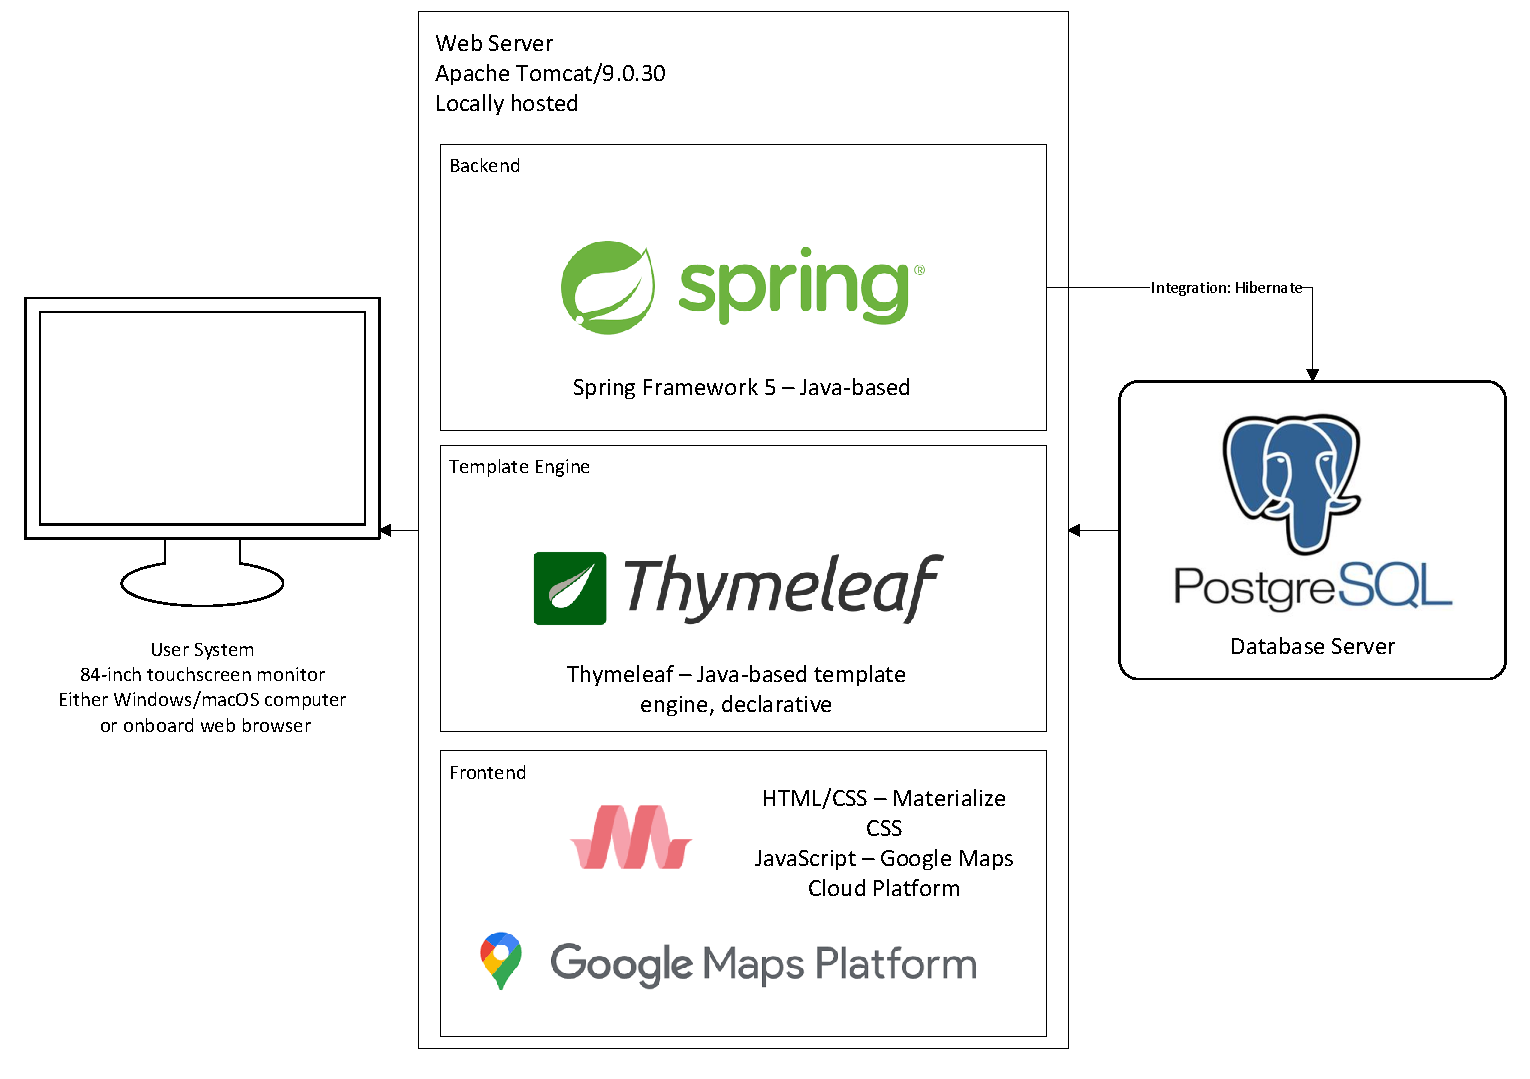
\includegraphics[scale=0.7]{diagrams/architecture_diagram}
	\caption{Architecture diagram for the Dyfi Wildlife Centre Web App}
\end{figure}	

Developing an architecture diagram ensured that there was a definition to the technology stack that the application is going to use. It also allowed for some prior thought to how different components interact with eachother.

For example, the database management system being used is PostgreSQL. Unlike systems such as SQLite, which is generally provided as a standalone file, PostgreSQL requires its own server instance. Therefore, research had to take place as to how the backend, running on Spring, would interface with the SQL Server. As evidenced in Figure 2.1, this was through Hibernate, an implementation of the standard Java persistence API for Spring's enterprise-level dialect. This was marked as something to research when planning the design for the model and controller layers of the backend.

The architecture diagram also identifies the relationships between each component hosted on the web server, in a downwards fashion. The Spring Framework interfaces with Thymeleaf, through Spring passing parameters to Thymeleaf templates, for them to be rendered. The frontend and user experience components of the application are clearly defined - with Materialize being used for the CSS layout, and the Google Maps Cloud Platform's JavaScript API being used for displaying the map and its markers. On the left-hand side, the user's system is explicitly mentioned, as User Experience is an important consideration in this project. The user will also be interacting directly with the system and its various components that are locally hosted on the web server.

\section{Database}

Parts of the database model were able to be generated automatically using the Spring Data JPA, however it was decided that a pre-built implementation of the database model would be easier to implement, as this would ensure adherence to an entity-relationship diagram, as well as any constraints that had been identified.

The initial iteration of the database, to fulfil the first two tasks that had been defined, was to have a single relation containing details about a point of interest. It was decided to initially plan the database in un-normalised form. This was to ensure that the Java object that was to be created in the back-end was readable and easy to maintain, rather than having to create multiple Java objects that represent a large number of relations in the database.

The database was to be iterated upon. To allow for authentication, separate tables for users and roles were to be created. While the consideration with regards to authentication was that every user should be automatically granted admin permissions, the role database allows for further addition of new roles, should this become a concern in a later version of the project.

\subsection{Entity-Relationship Modelling}
\begin{figure}[H]
	\caption{Second iteration of the Dyfi Wildlife Centre schema}
	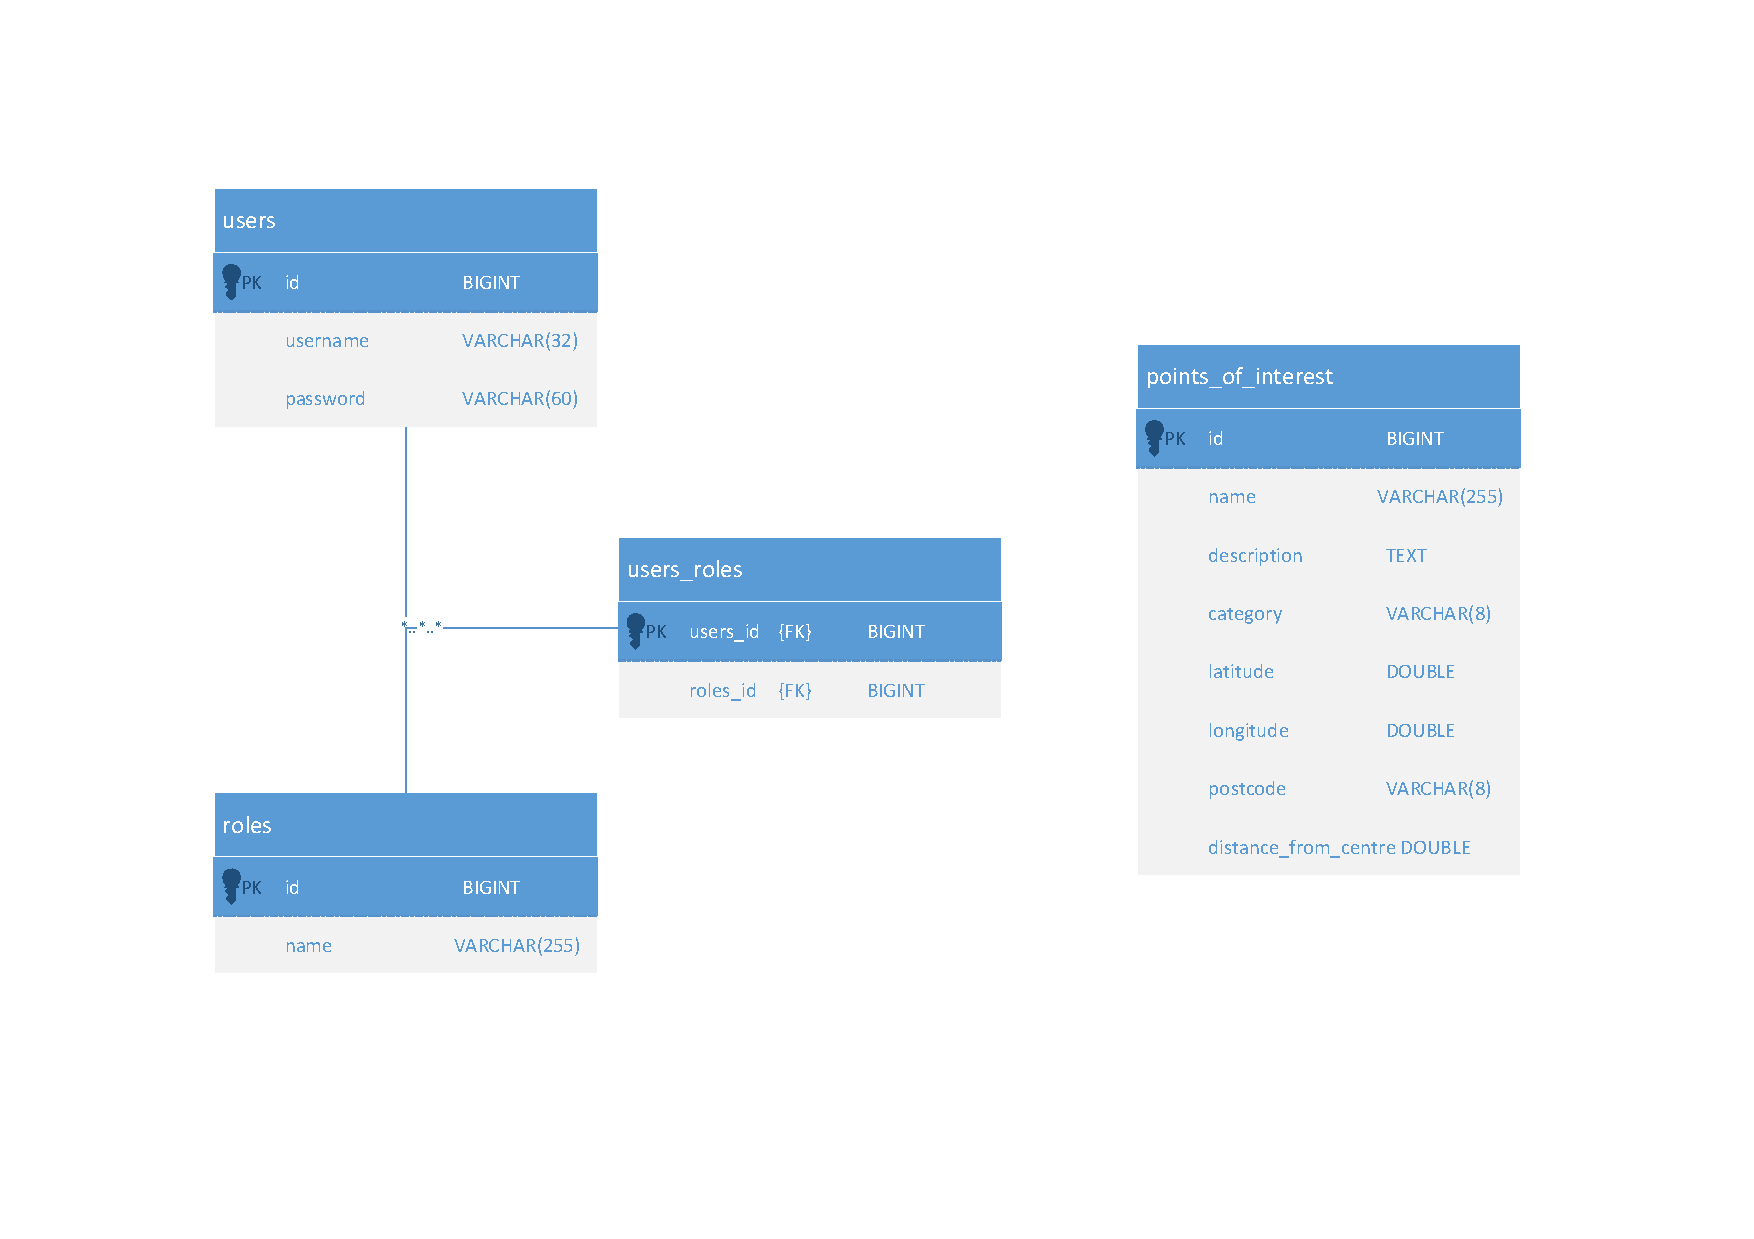
\includegraphics[scale=0.6]{diagrams/er_diagram}
\end{figure}	

Ultimately, the database design was uncomplicated, as there were only three objects to consider. As the majority of database handling was intended to be carried out through the Spring Data JPA, the nuances that that brings were added into the database at time of design. One example would be the ID primary key on each relation. In a standard PostgreSQL database implementation, the data type of the ID is not likely to be of type \textit{bigint}. This is a type that is, as the name implies, intended for large integers. An ID attribute that is being utilised as a primary key would generally take the type of \textit{serial} - an auto-incrementing column. This is, however, handled within the backend by the JPA, through an automatically-generated sequence stored within the database, therefore there is no need to use the serial type.

It is also true that, in a standard database, there would be an argument for not having an automatically-generated primary key, and instead using another unique property, such as name, or a compound primary key. However, this implementation was chosen as it allowed for faster efficiency within the backend layer of the application - a primitive type would be able to be matched faster than a String object with a string-matching algorithm behind it.

A many-to-many relationship between both users and roles is achieved through the use of a junction able, \textit{users\_roles}. This allows for multiple roles to be added into the database at a later date, which can then be attributed to users through the frontend. As each user is only permitted to have one role, the primary key has been set as the user in the junction table, with a role ID being set with each user.

\subsection{Constraints}

Constraints had to be created in order to validate the data that was being entered into the table, this is described below, with the definition in a pseudo-code format:

% Please add the following required packages to your document preamble:
% \usepackage{graphicx}
\begin{table}[H]
\centering
\resizebox{\textwidth}{!}{%
\begin{tabular}{|l|l|}
\hline
\textbf{Constraint Name}                   & \textbf{Definition}                                    \\ \hline
\textbf{latitude\_chk}                     & CHECK latitude IS \textgreater -90 AND \textless 90    \\ \hline
\textbf{longitude\_chk}                    & CHECK longitude IS \textgreater -180 AND \textless 180 \\ \hline
\textbf{latitude\_not\_null\_island\_chk}  & CHECK latitude NOT EQUAL TO 0                        \\ \hline
\textbf{longitude\_not\_null\_island\_chk} & CHECK longitude NOT EQUAL TO 0                        \\ \hline
\textbf{chk\_name}                         & CHECK name IS NOT EMPTY                                \\ \hline
\textbf{postcode\_chk}                     & CHECK postcode MATCHES UK postcode regex               \\ \hline
\end{tabular}%
}
\caption{A list of constraints in the points\_of\_interest relation}
\label{poi_constraints}
\end{table}

These constraints tend to perform sanity checks on the input that is being entered, once it reaches the database layer. The constraints on the coordinates are based upon the natural constraints based upon latitude and longitude, and ensures that a user cannot apply an incorrect coordinate to a point of interest, that would likely cause an error at the frontend layer of the application.

The two ``not null island" checks make sure that a user cannot simply enter 0 as the latitude and 0 as the longitude, as this could potentially cause issues when parsing the postcode in the backend layer. The primary issue with a check like this would be that 0,0 is a valid coordinate pair. However, the customer has specified that points of interest would primarily be in the United Kingdom, which is far from this coordinate range. It is not likely that any potential coordinate pairs entered for points of interest outside the UK would be equal to these coordinates.

A regular expression, sought from an open data source that provides APIs dealing with UK postcodes\cite{PostcodeRegex}, was, again, a sanity check. It performs basic error-checking that checks the general shape of the postcode; checking it has a letter at the beginning and ends in a letter, for example. Stricter regular expressions were available, however improvements were marginal and an API to confirm the postcode was valid was still required, due to the inability for a regular expression to rule out false positives. The design accounts for error-checking of postcodes through the use of the aforementioned API, which is further explained in section~\ref{sec:backend}. 


\section{Backend}
\label{sec:backend}

\begin{figure}[H]
	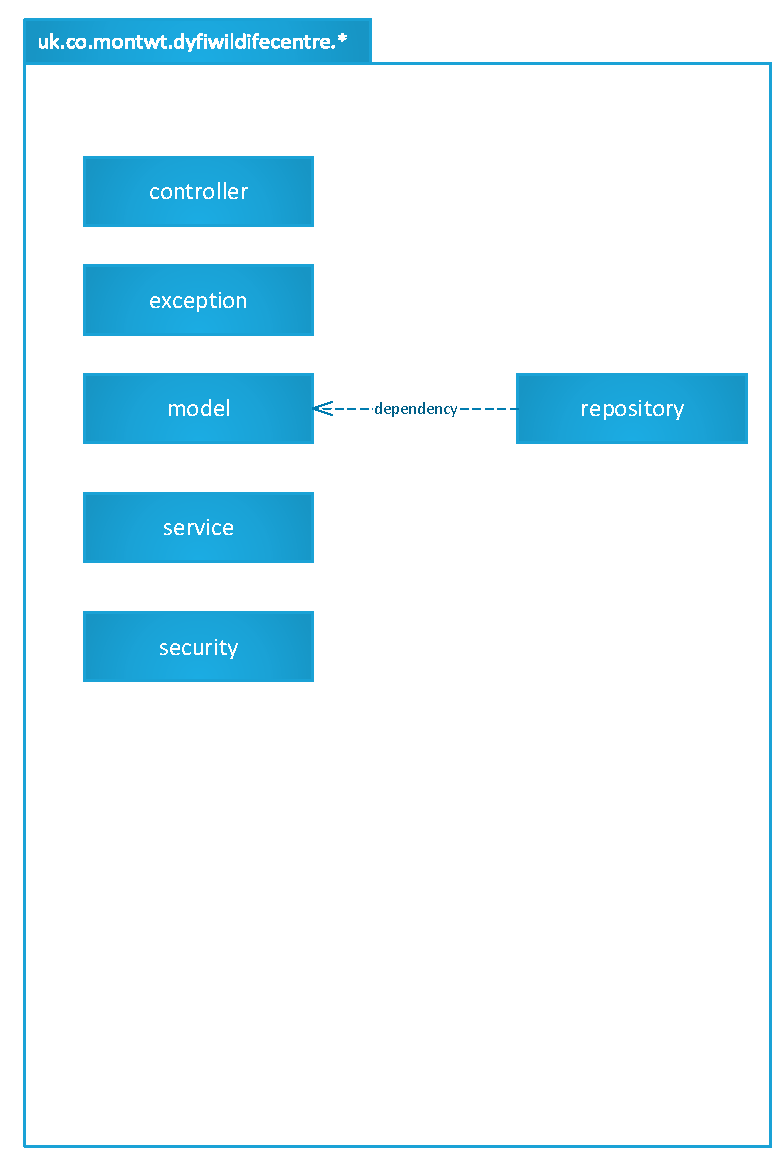
\includegraphics[scale=0.7]{diagrams/parent_uml}
	\caption{Parent UML diagram, showing each package that the software breaks down into}
\end{figure}	

Spring, the framework that is utilised in this backend, follows a model-view-controller design pattern. This allows for a clear distinction between each area of the application, with its functionalities and design being defined as follows:

\begin{itemize}
	\item	\textbf{Model} - The application's data structure and logic processing, containing the objects representing a user, a role, and a point of interest. It also includes a repository layer, that interfaces with the PostgreSQL server, and a service layer, that provides a layer of abstraction between the database and the controller.
	\item	\textbf{View} - The presentation of data in the application. This is generally further discussed in Section~\ref{sec:frontend}.
	\item	\textbf{Controller} - Classes that accept user and computer input, converting it to commands that affect either the model or the view. In this application, the controller consists of a RESTful API for managing users and points of interest.
\end{itemize}

Class diagrams were created to be adhered to during the production of this application, and were split by layer. For the sake of clarity; constructor, setter, and getter methods are not represented on the class diagram. The intention was for Java packages to be used, to aid in code navigability and ease of maintenance.

\subsection{Model layer}
\begin{figure}[H]
	\includegraphics[scale=0.7]{diagrams/model}
	\caption{Class diagram of the \texttt{uk.co.montwt.dyfiwildlifecentre.model} package}
\end{figure}	

The primary model layer contains one class, as well as a sub-package. The sub-package contains an interface that accesses the \textit{point\_of\_interest} relation in the database, utilising a Spring Data JPA superclass. It contains one method, that is intended to invoke an SQL command directly that finds a point of interest by its name, rather than its ID.

The \texttt{PointOfInterest.java} class defines a point of interest in an identical fashion to that of the database layer. This is required by the Spring Data JPA, and results in fewer manual configurations to be carried out. It was noted that a refactoring of this class diagram could include a further class, named Location, that includes the location-based members of PointOfInterest. This could be represented in the database by a one-to-one relationship. However, at least initially, this was not to be represented in the data modelling, and as the project is being developed in an agile fashion could be refactored in the future if considered necessary.

The \texttt{calculateDistanceFromCentre()} is designed such that it calculates the great-circle distance between two pairs of coordinates, with one being the coordinates for the Dyfi Wildlife Centre. This calculation would be in miles, to four significant figures, and would help in presenting users the distance between points of interest and the visitor centre. The \textit{Haversine formula}, a formula in spherical trigonometry to determine distance between two points on a sphere, was to be implemented, with the code that was used available in Appendix C, section~\ref{haversine}. Although the Earth is not a perfect sphere, Haversine's formula provides an acceptable approximation of distance between two points, taking into account the short distances that the user's requirements specify.

\subsection{Controller Layer}

The controller layer at this level of the application is intended to act as a RESTful API that interfaces with a point of interest and its database. Therefore, the HTTP requests that surround the API are intended to be as clear as possible as to their intention with as much avoidance of side-effects as possible. The controller layer also includes a sub-layer, to interface between itself and the database.

\subsubsection{Services}
\label{geocoding}
\begin{figure}[H]
	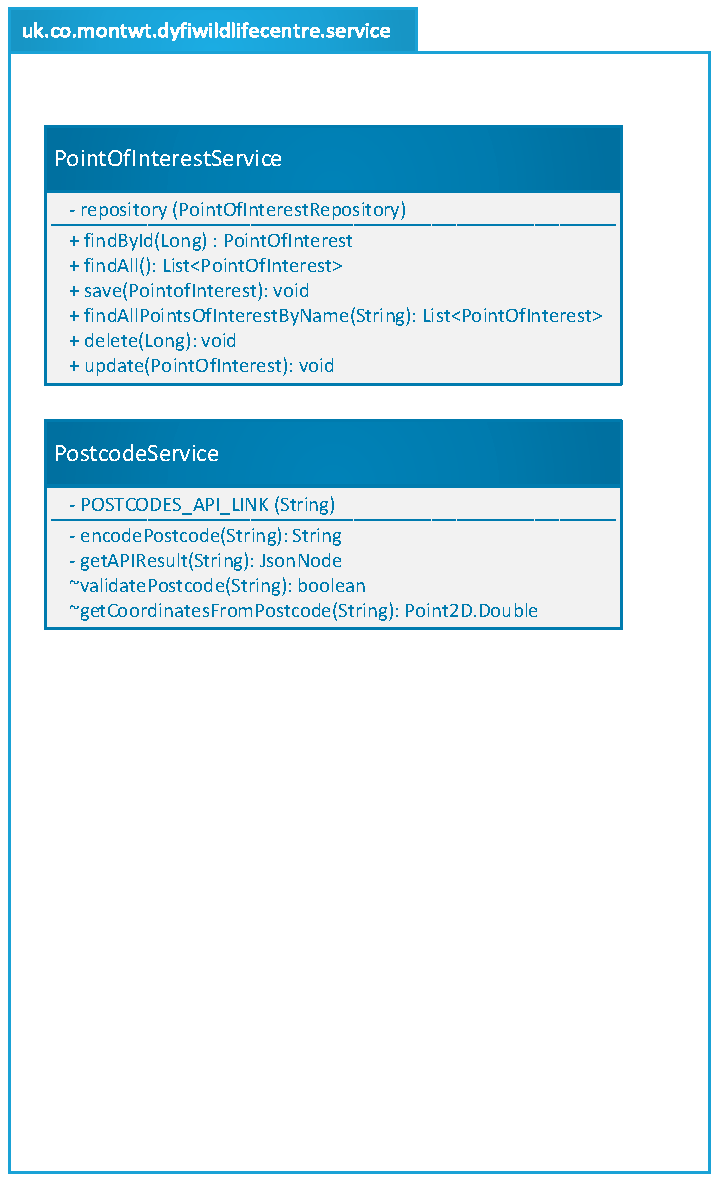
\includegraphics[scale=0.7]{diagrams/modelservice}
	\caption{Class diagram of the \texttt{uk.co.montwt.dyfiwildlifecentre.service} package}
\end{figure}	

The controller layer of this application utilises a service layer - providing an extra layer of abstraction between the database and the controller. It also includes any logic required within the methods, for example, any backend-level error-checking before the object is passed to the database.

The \texttt{PointOfInterestService.java} class manages the data transferring between the controller layer, the model layer, and the database. Method such as \texttt{findAll()} and \texttt{delete(Long id)} simply make a method call to an identical repository method, that manages the SQL transaction. However, some other methods are slightly more complicated, the most prominent example being the \texttt{save(PointOfInterest poi)} method. The method first determines if a postcode or a coordinate pair was entered into the form. If a postcode was entered, then a method call must be made to fetch the coordinates corresponding to that postcode. If not, there is no need to, however an error will occur if both a postcode and coordinates had been entered. The distance from the centre is also calculated and set in the object, before it being passed to the database.

The second service, \texttt{PostcodeService.java} manages parsing of postcodes, and includes methods to both validate a postcode, and get the coordinates that correspond to a postcode. This utilises the `postcodes.io` API, an open-source, RESTful API that utilises open data primarily provided by the Ordnance Survey, the United Kingdom's national mapping agency\cite{PostcodesAPI}. Methods in this service are used to validate a postcode - ensuring that it is a real postcode and there is information available for it, as well as looking up a postcode and extracting the given latitude and longitude. This will not be an exact location, particularly if the user is marking a place on a residential street, for example. However, coordinates can still be added manually if more precision is required, and a postcode will still provide visitors an idea of where the point of interest is. Other APIs, such as the geocoding API included in Google Maps Platform, were considered, however further analysis of the pricing model saw that there was a risk of utilisation of such an API being costly.

\subsubsection{Controllers}
\begin{figure}[H]
	\includegraphics[scale=0.6]{diagrams/controller}
	\caption{Class diagram of the \texttt{uk.co.montwt.dyfiwildlifecentre.controller} package}
\end{figure}	

There are three controllers within this layer of the application, each with three distinct responsibilities.

The \texttt{MvcConfig.java} package is designed such as to reduce the number of methods required for simple loading of a view, with other methods designed to either include a payload in its model or related directly to the API that the controller is implementing. The class has only one method, that declaratively adds a view controller with a URL path, along with the correct view name.

\texttt{AdminController.java} controls data that is being passed to the admin panel view models, with the methods within the controller either carrying objects within its model, or having a model passed to it via a query string that is appended to the URL. Continuing with the abstraction granted through the service layer, the methods are short, simply adding attributes to the model for them to be handled in the view.

\texttt{PointOfInterestController.java} has a greater number of methods, that handle requests as a RESTful API. A brief specification is included in the table below.

% Please add the following required packages to your document preamble:
% \usepackage{graphicx}
\begin{table}[H]
\centering
\resizebox{\textwidth}{!}{%
\begin{tabular}{|l|l|l|}
\hline
\textbf{Endpoint}    & \textbf{Description}                                                                      & \textbf{Return Type}                         \\ \hline
/poi/get/id/:id      & Returns the point of interest where :id corresponds to the ID of the point of interest     & PointOfInterest                              \\ \hline
/poi                 & Returns all points of interest in the database                                            & List\textless{}PointOfInterest\textgreater{} \\ \hline
/poi/form\_create?poi=:poi &
  Saves a point of interest to the database where :poi corresponds to the point of interest to be saved &
  RedirectView \\ \hline
/poi/get/name/:name &
  Returns the points of interest where :name corresponds to the name of the point of interest &
  List\textless{}PointOfInterest\textgreater{} \\ \hline
/poi/delete?id=:id   & Deletes the point of interest where :id corresponds to the ID of the point of interest    & RedirectView                                 \\ \hline
/poi/update?poi=:poi & Updates a point of interest where :poi corresponds to the point of interest to be updated & RedirectView                                 \\ \hline
\end{tabular}%
}
\caption{API endpoints for /poi}
\label{tab:poi-endpoints}
\end{table}

Whilst RESTful values were adhered to as much as possible, HTML's incompatibility with request that are not GET or POST required methods such as delete to be HTTP GET request rather than HTTP DELETE. This will be further discussed in the Implementation chapter.


\subsection{Security}
\label{springpassword}

Various information security considerations had to be taken into account whilst designing the application, the main one being authenticating and securing the administration panel. As the software is designed for use in a public location, an unauthenticated admin panel, where anybody who wants to could add or edit points of interest and users, was not acceptable. Therefore, a strategy for user authentication had to be put into place.

An example of a threat affecting the authentication of the application, once implemented, could be an SQL injection. A successful attack could expose user passwords and tamper with existing data stored in the database. If an attacker was able to gain access to the wireless network that the customer will be connecting the system to, they may be able to connect to the database remotely, resulting in physical limitations on access to hardware becoming futile. A suggestion could be made to the customer to secure their wireless network, perhaps having one SSID for public use and one for private use, however there is no way to enforce this in the application. With the application being hosted locally, it would be difficult to encrypt requests via HTTPS without creating a standalone server.

To combat these security concerns, Spring Security, an authentication framework designed for use with Spring, was implemented, through the contents of the security package. Users were stored in an SQL database, along with their roles. The default authentication method for users was plain-text, and users passwords could be easily found in the database. This was modified to use ``bcrypt", a password hashing function based upon the Blowfish cipher\cite{bcrypt}. bcrypt hashes the password that the user has been registered with, and then stores that hash in the password field of the relation. When a user logs in, the password that has been provided is matched against the hash, rather than the hash being decrypted, resulting in it not being reasonably possible to crack a password from the hash. 

\subsubsection{Model layer}
\begin{figure}[H]
	\includegraphics[scale=0.7]{diagrams/security/model}
	\caption{Class diagram of the \texttt{uk.co.montwt.dyfiwildlifecentre.security.model} package}
\end{figure}

The model layer of the security package implements the database. There are no special methods and the purpose is simply to represent the database as Java objects.

\begin{figure}[H]
	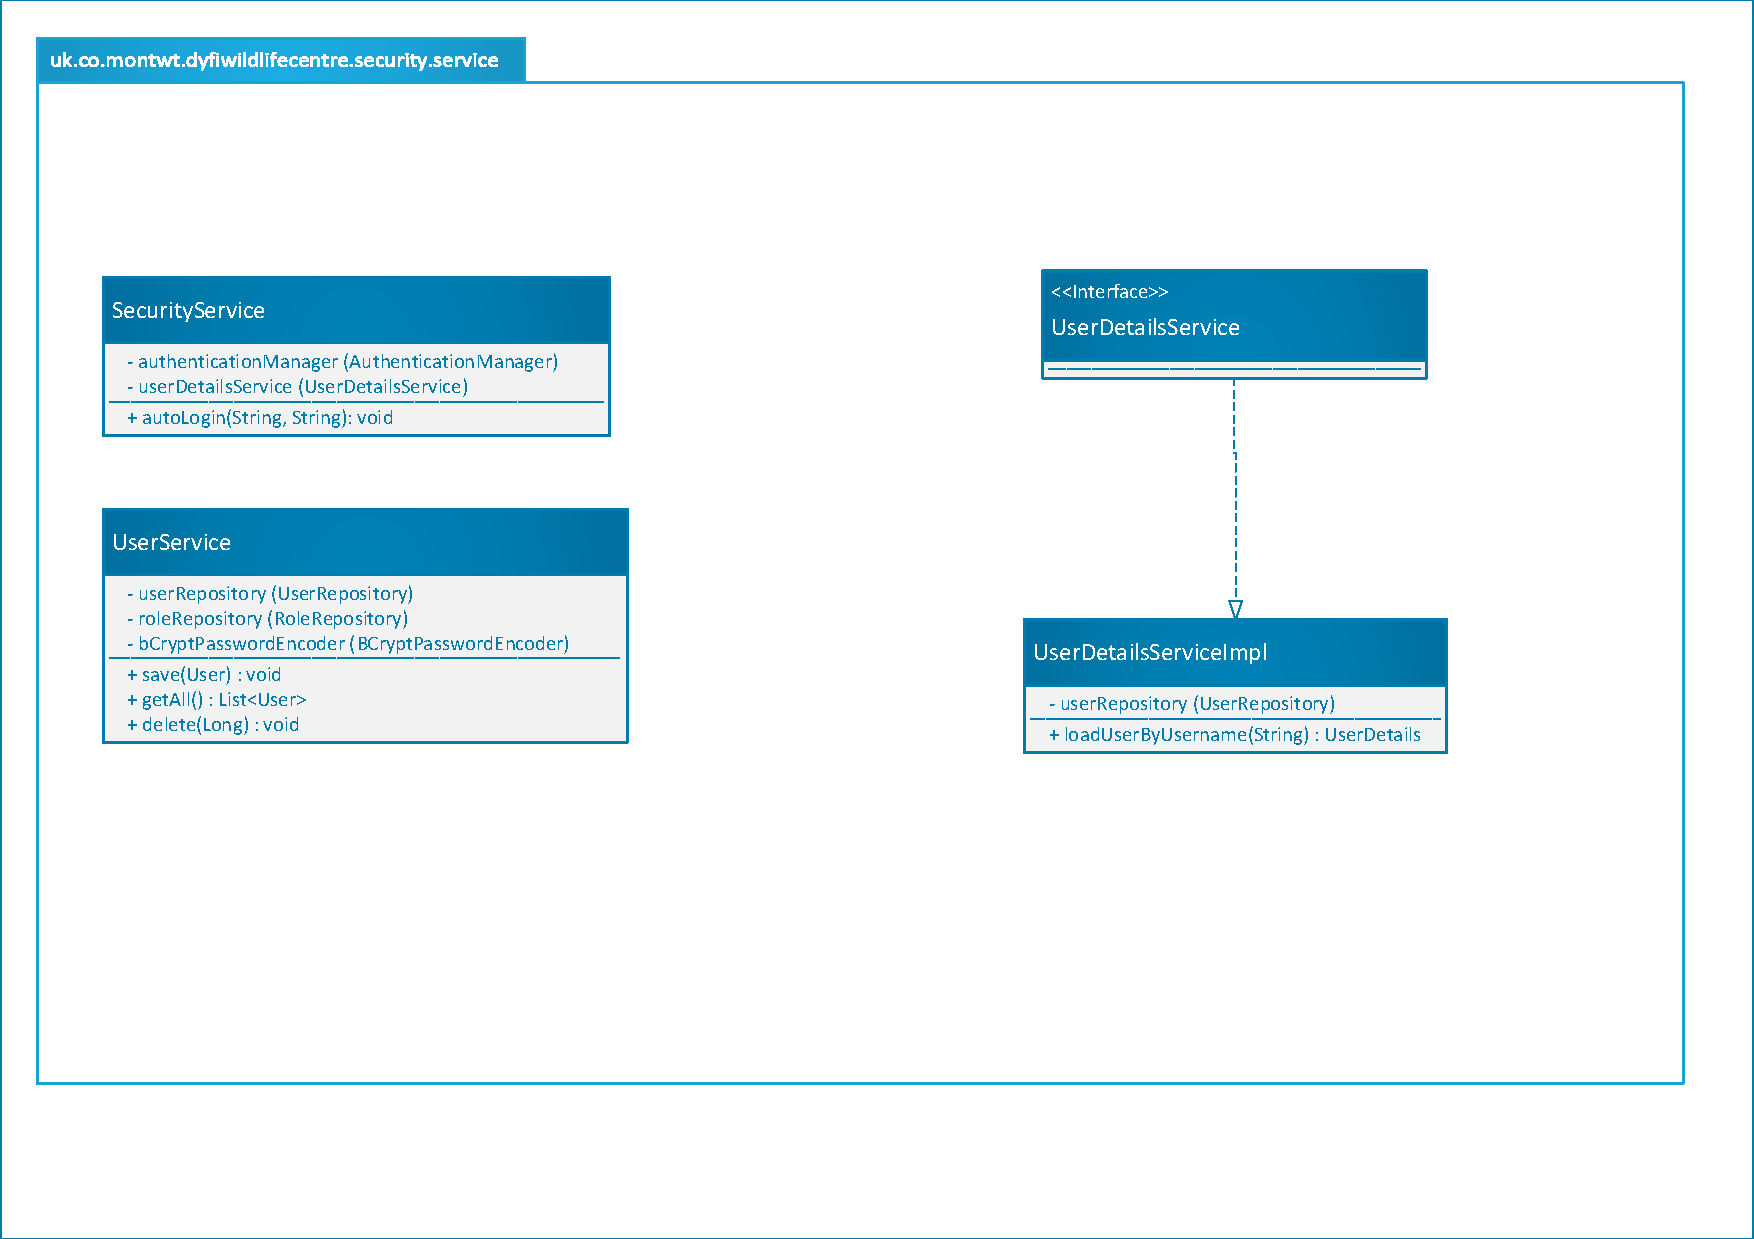
\includegraphics[scale=0.6]{diagrams/security/service}
	\caption{Class diagram of the \texttt{uk.co.montwt.dyfiwildlifecentre.security.service} package}
\end{figure}

The security layer contains implementations for an interface from the Spring Security package, as well as instantiating Spring Security's authentication manager. In the \texttt{save(User user)} method in \texttt{UserService.java}, the BCrypt encoder is called, and the password is encrypted. As discussed above, the password is sent to the service in plain text, however this would be difficult to encrypt without HTTPS, and data transfer is being carried out solely on the local host due to the nature of the locally hosted database.

\subsubsection{Controller layer}
\begin{figure}[H]
\includegraphics[scale=0.7]{diagrams/security/controller}
\caption{Class diagram of the \texttt{uk.co.montwt.dyfiwildlifecentre.security.controller} package}
\end{figure}

The controller layer of the security package includes a RESTful controller as well as a controller for the User object itself, that, as with the PointOfInterestController, interfaces with the service and the database. \texttt{UserRestController} implements a GET request, that returns all users, in order for them to be displayed in a list. \texttt{UserController} manages the registration and deletion of users, containing method calls to the relevant services. It also includes an exception handler, that reports a conflict message to the user, should they attempt to register a user with the same username as one that has already been registered.

\section{Frontend}
\label{sec:frontend}

\subsection{Design considerations}

The frontend is a crucial part of this application, as this will be what the end user will be viewing. There were some key considerations that had to take place when making decisions regarding how to design the User Experience.

Familiarity was an important consideration to make, as users may not have a large amount of technical training, and a layout that they would be used to from different applications may be beneficial. This was part of the reasoning behind choosing Material Design as the design language for this software - with most Android, and some iOS apps, using Material Design, as well as popular web services such as Google Maps, there would not be a large number of potentially confusing prompts and dialogues.

An aspect of minimalism was required with the design of the software, particularly on the homepage. The core function of the software was to show points of interest on a map, and having too many other UI components on the front page could potentially result in the page being too bloated. There was not too much of a need for a change from this in the admin panel, with clear instructions as to what the purpose of the view was.

Inspiration from the design came from similar web applications, which had a map as its main centrepiece. An example of a site assessed is the Airbnb accommodation-booking website\cite{airbnb}. This website uses a clear, relatively minimalistic, design. It is clear that, when searching for accommodation, its main element is a map, that includes markers and some options for filtering the map. This added to the strategy used within the frontend, and the inclusion of distinct, clickable markers.

Another website that was evaluated prior to design of the frontend was an element of Rightmove's website, a website intended to find property to buy or rent\cite{rightmove}. In the cited example, it was noted that an action bar took a small section of the top part of the page, with the map taking the majority of the page. Whilst markers differ in this implementation, with Materialize's modal design being used to hold a card as opposed to a sidebar being opened, inspiration from Rightmove was taken as to the prominence of the map and the lack of any distractions.

\subsection{Prototyping}

Prototyping and mockups were created as part of the planning and design process. These mockups were based on Semantic UI, which was changed to Materialize after the mockups were created. As there were quite a few similarities, it was decided to not redesign the mockups.

\subsubsection{Home Screen}
\begin{figure}[H]
\includegraphics[scale=0.2]{mockups/Home Screen}
\caption{Home Screen mockup}
\end{figure}

The initial representation of the home screen showed a menu bar, at the top of the page, along with a hamburger menu. The main component of the home screen was the Google Maps component, with filter and reset buttons on either side of it. The general shape of this mockup was carried over to the final build, however a floating action button was used in place of two distinct buttons.
\newpage
\subsubsection{Marker information}
\begin{figure}[H]
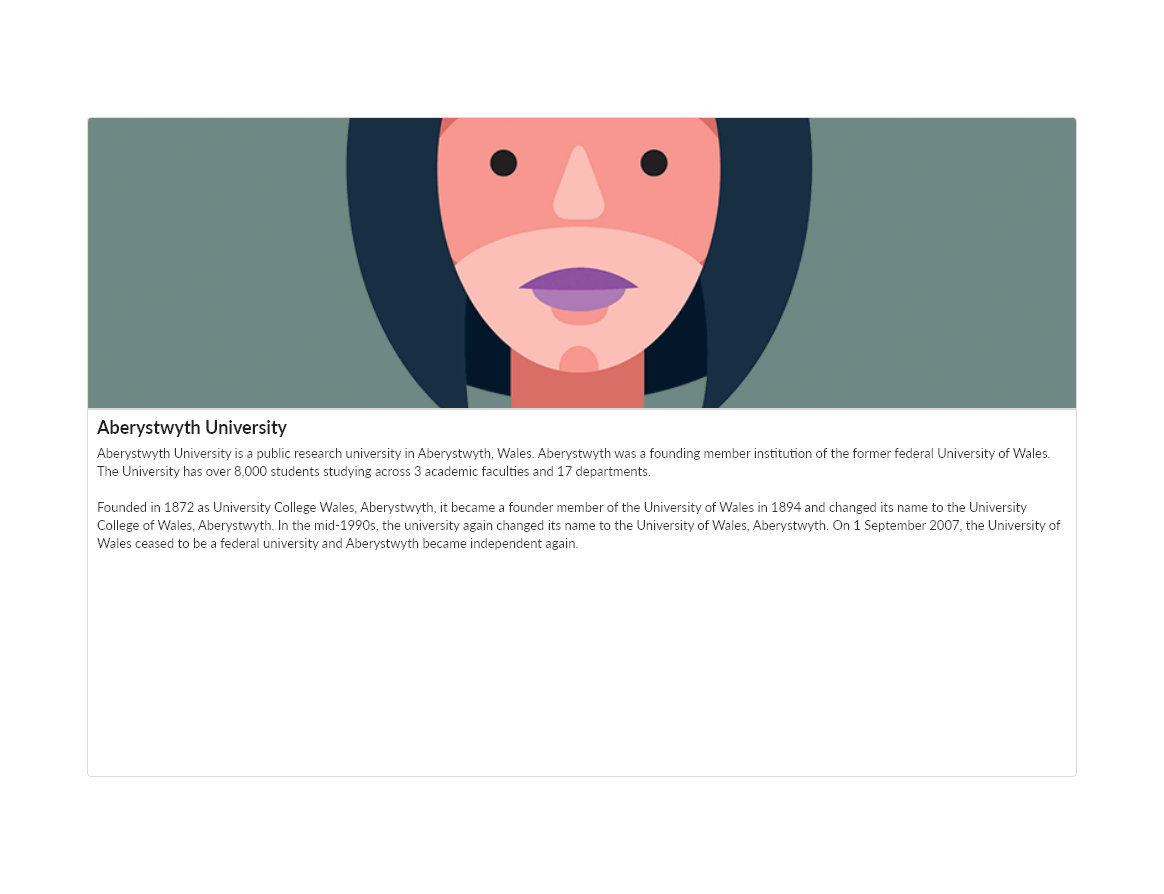
\includegraphics[scale=0.2]{mockups/POI card}
\caption{Mockup of the POI card}
\end{figure}

The `POI card` was designed such that it would contain easily-readable information, including a title, a description, and a relevant image. The POI card appears should a user click on a marker, with the JavaScript function for the Maps API being used to populate these fields. The scripts used to show the POI card are available in Appendix C.

\subsubsection{Admin Panel - Login Screen}
\begin{figure}[H]
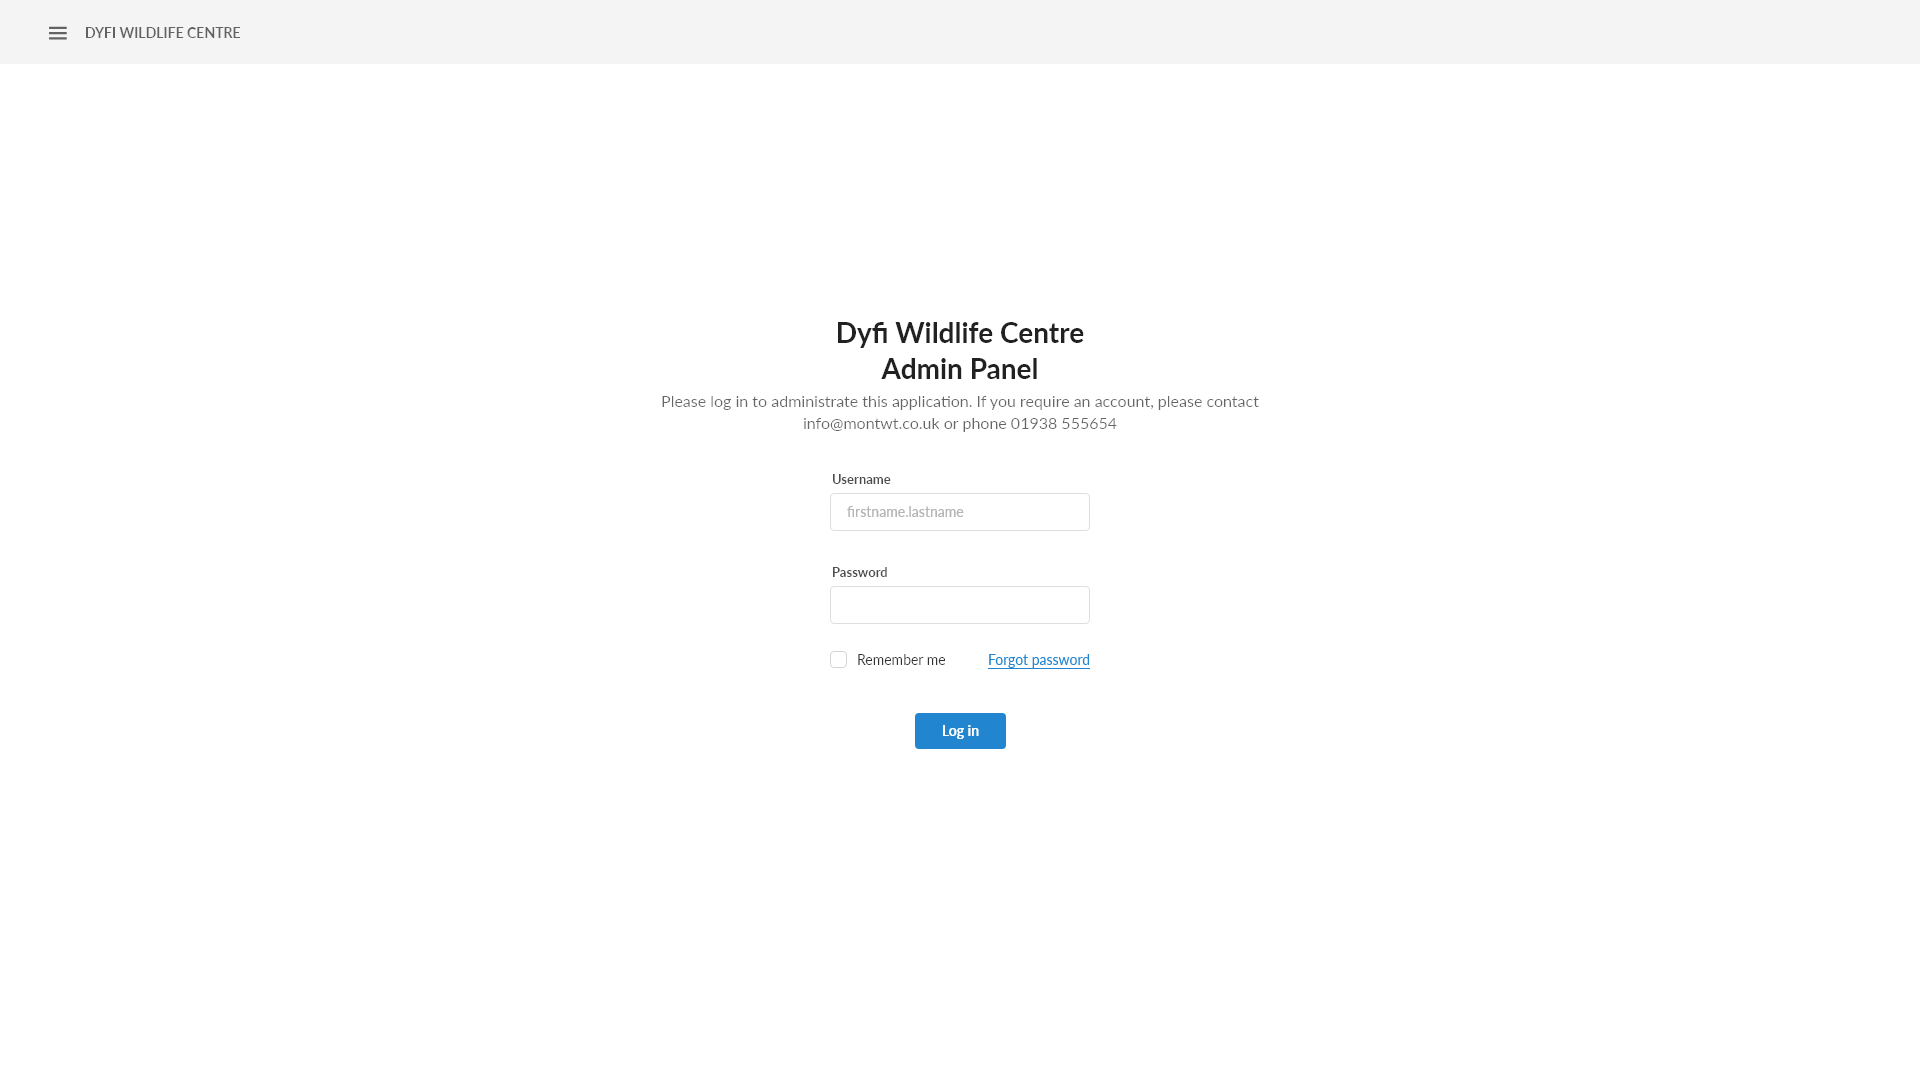
\includegraphics[scale=0.2]{mockups/Admin login screen}
\caption{Mockup of the admin login screen}
\end{figure}

As explained above, the admin login screen was designed to be as minimalistic as possible. It simply includes a username and password, as well as a brief piece of information describing how one would go about requesting a login for the admin panel. Spring Security is used to facilitate the login.

\subsubsection{Admin Panel - POI editing}
\begin{figure}[H]
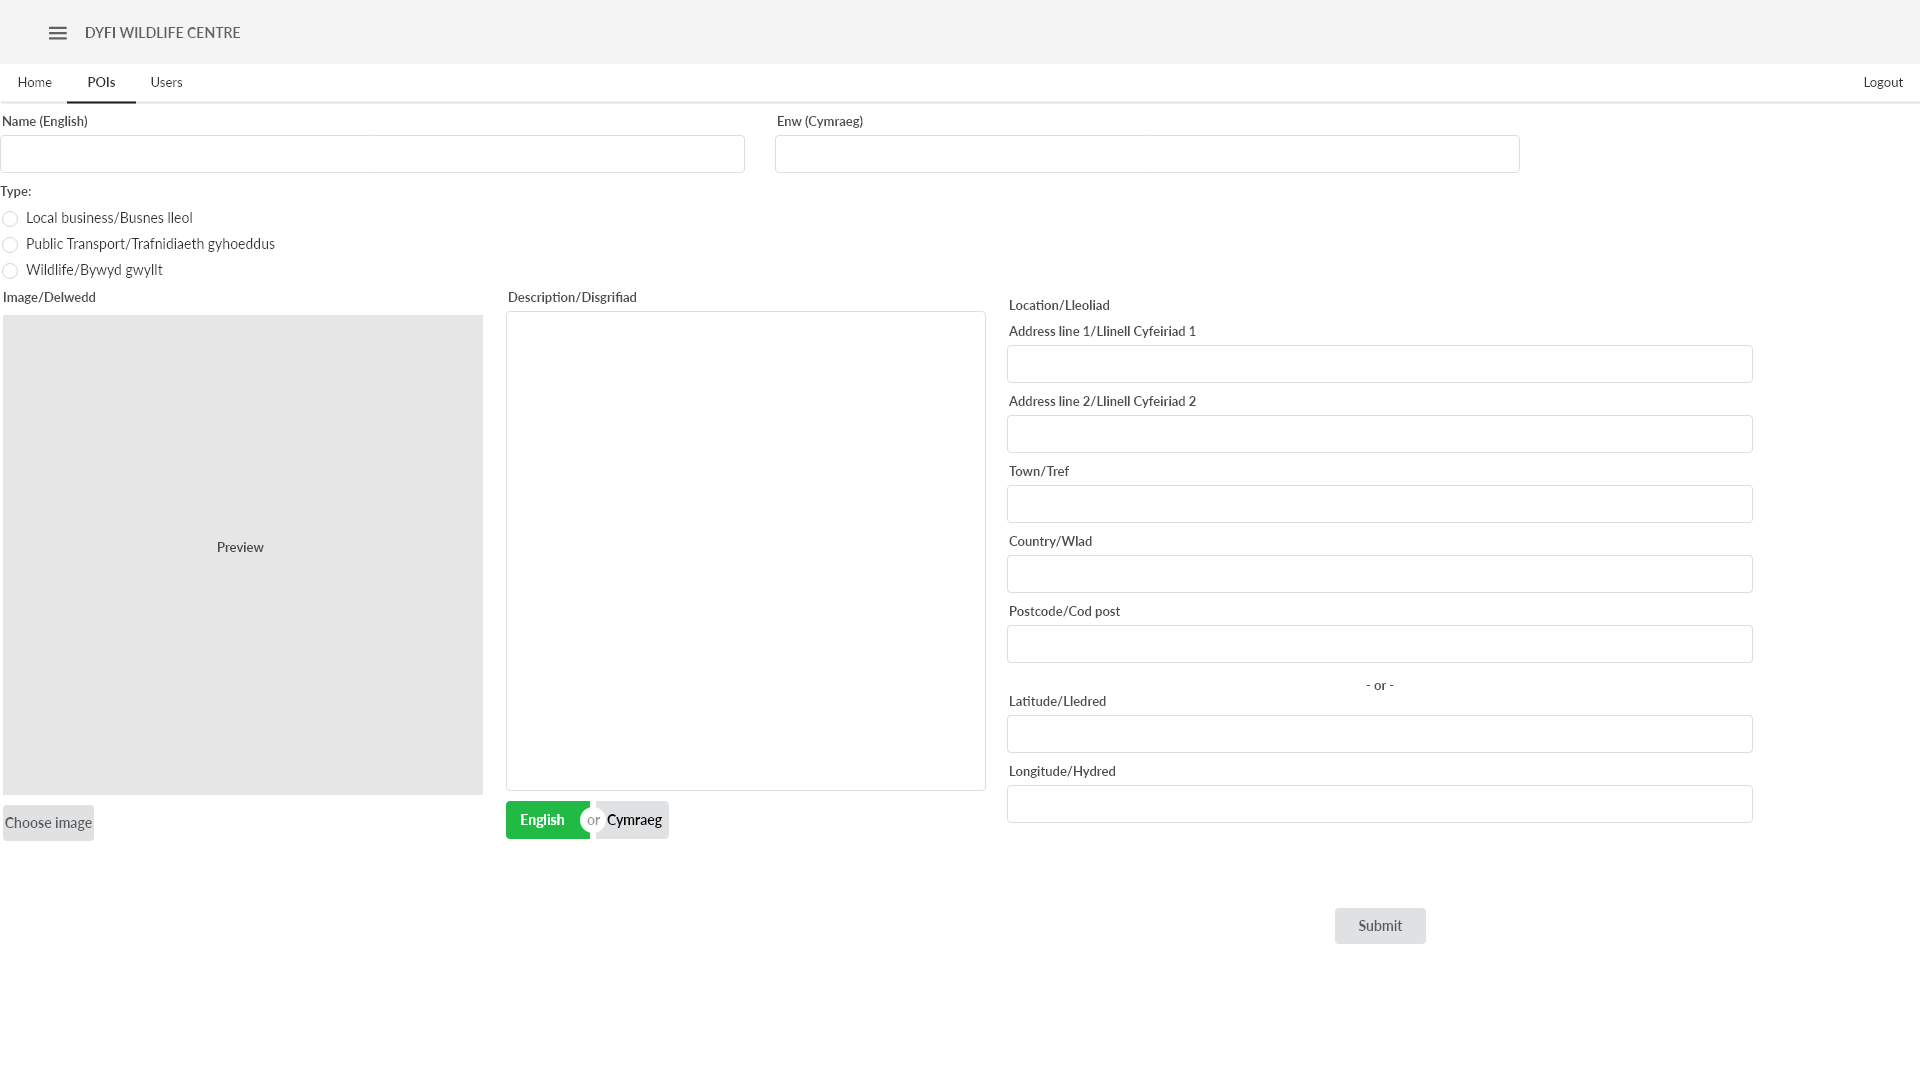
\includegraphics[scale=0.2]{mockups/Admin Panel - POIs (not filled, English)}
\caption{Mockup of the POI editing prompt}
\end{figure}

The initial logic behind the POI editing screen allowed for an entire address to be added, and a coordinate pair if it was deemed necessary by the user. Ultimately, this was considered an overcomplicated solution, and, as explained above, either a postcode or a coordinate pair were required.
\newpage
\subsubsection{Admin Panel - User management}
\begin{figure}[H]
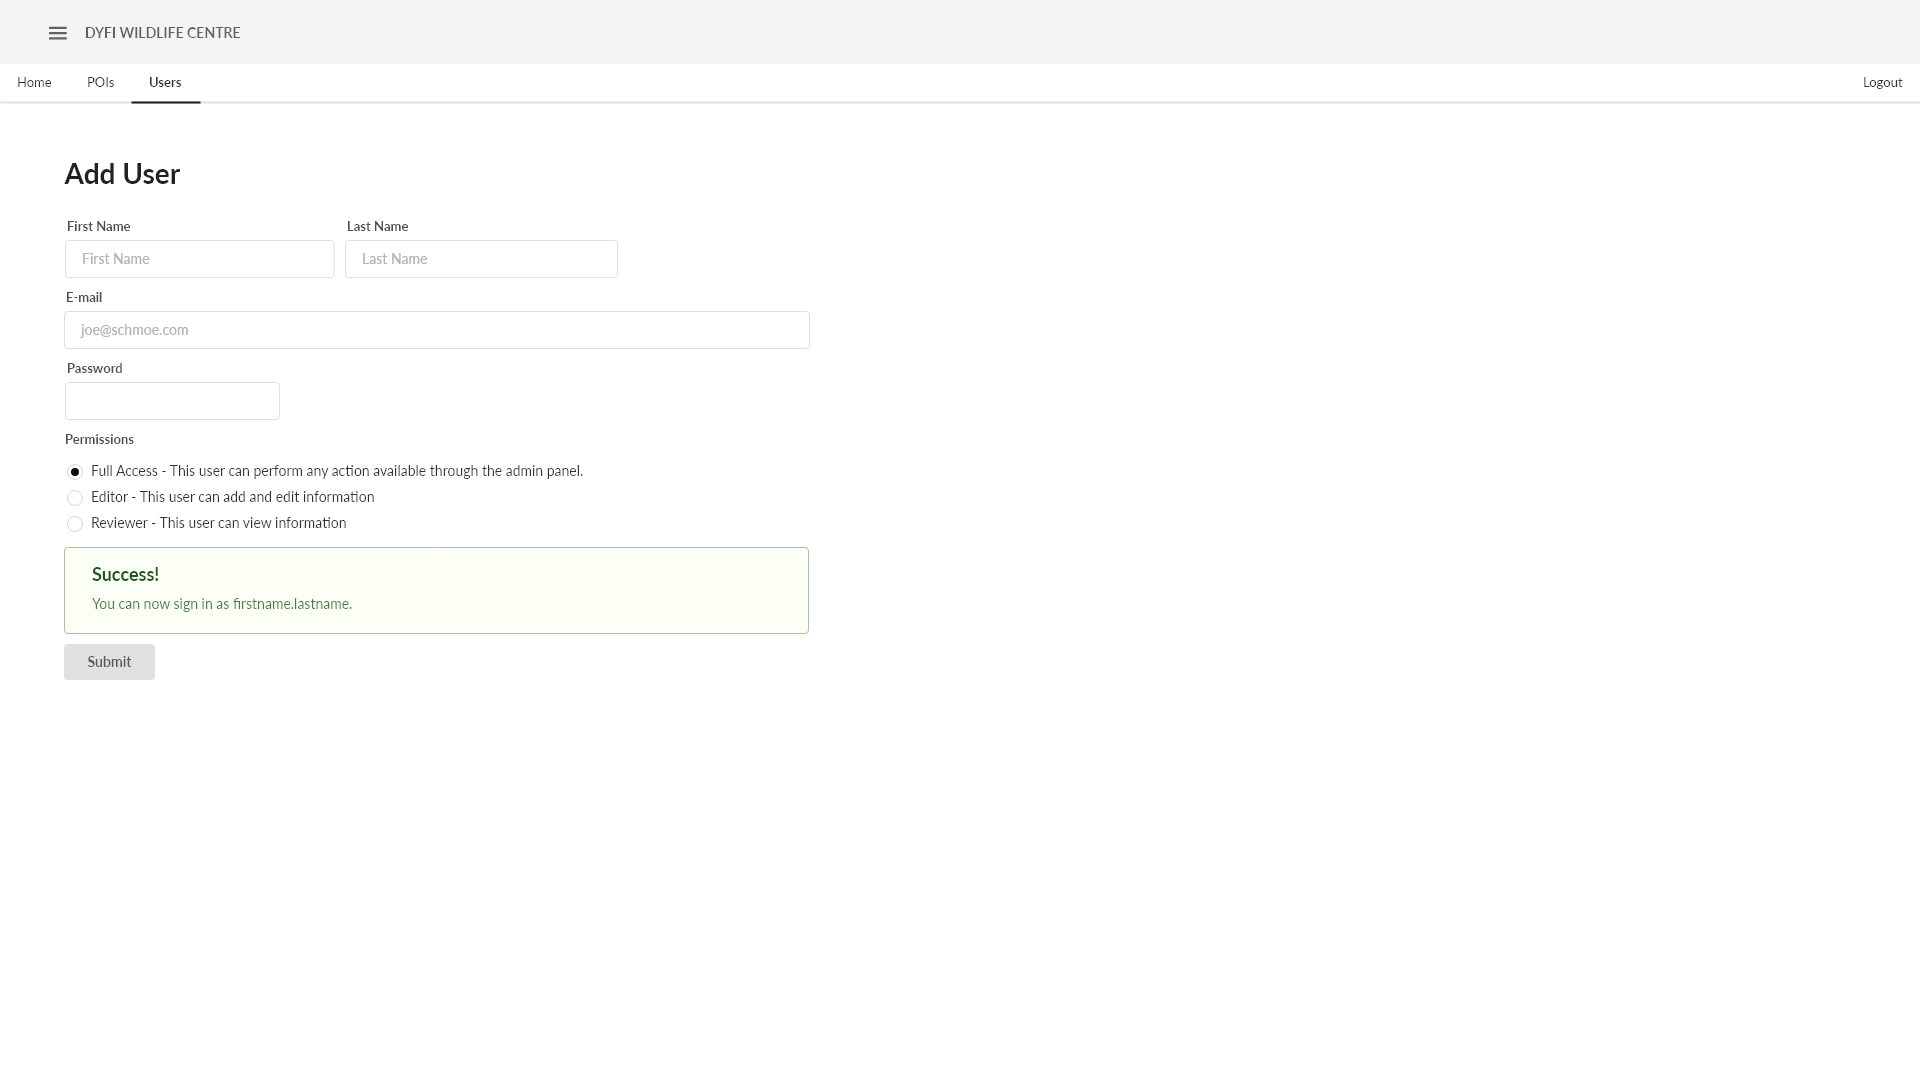
\includegraphics[scale=0.2]{mockups/Admin Panel - Add User}
\caption{Mockup of the 'Add a user' screen}
\end{figure}

Similarly, adding a user with various details was later decided to be redundant, as a simple username and password would suffice for security purposes. Changes in decisions made will be discussed in Chapter 3.

% Word count: 3454
\chapter{Software Design, Implementation and Testing}

This could be one chapter or a few chapters. It should define and discuss the software that is developed to support the research that is being conducted. For example, if your research involves running experiments, what software are you creating to support that work? What functionality is required? What design will be used? What implementation issues are there and what testing is used? 

Even though a research project is investigating specific research questions, it is still necessary for you to discuss the software that you develop. Research has a habit of generating bits of software that can exist for several years and need future modification. Therefore you need to be able to discuss the technical issues as well as the research approach. 

\section{Design}
You should concentrate on the more important aspects of the design. It is essential that an overview is presented before going into detail. As well as describing the design adopted it must also explain what other designs were considered and why they were rejected.

The design should describe what you expected to do, and might also explain areas that you had to revise after some investigation.

Typically, for an object-oriented design, the discussion will focus on the choice of objects and classes and the allocation of methods to classes. The use made of reusable components should be described and their source referenced. Particularly important decisions concerning data structures usually affect the architecture of a system and so should be described here.

How much material you include on detailed design and implementation will depend very much on the nature of the project. It should not be padded out. Think about the significant aspects of your system. For example, describe the design of the user interface if it is a critical aspect of your system, or provide detail about methods and data structures that are not trivial. Do not spend time on long lists of trivial items and repetitive descriptions. If in doubt about what is appropriate, speak to your supervisor.
 
You should also identify any support tools that you used. You should discuss your choice of implementation tools - programming language, compilers, database management system, program development environment, etc.

Some example sub-sections may be as follows, but the specific sections are for you to define. 

\subsection{Overall Architecture}

\subsection{Some detailed design}

\subsubsection{Even more detail}

\subsection{User Interface}

\subsection{Other relevant sections}

\section{Implementation}

This section should discuss issues you encountered as you tried to implement your experiments. What were the results of running the experiments? What conclusions can you draw from these results? 

During the work, you might have found that elements of your experiments were unnecessary or overly complex; perhaps third-party libraries were available that simplified some of the functions that you intended to implement. If things were easier in some areas, then how did you adapt your project to take account of your findings?

It is more likely that things were more complex than you first thought. In particular, were there any problems or difficulties that you found during implementation that you had to address? Did such problems simply delay you or were they more significant? 

If you had multiple experiments to run, it may be sensible to discuss each experiment in separate sections. 

\section{Testing}
Detailed descriptions of every test case are definitely not what is required in this section; the place for detailed lists of tests cases is in an appendix. In this section, it is more important to show that you adopted a sensible strategy that was, in principle, capable of testing the system adequately even if you did not have the time to test the system fully. 

Provide information in the body of your report and the appendix to explain the testing that has been performed. How does this testing address the requirements and design for the project?

How comprehensive is the testing within the constraints of the project?  Are you testing the normal working behaviour? Are you testing the exceptional behaviour, e.g. error conditions? Are you testing security issues if they are relevant for your project?

Have you tested your system on ``real users''? For example, if your system is supposed to solve a problem for a business, then it would be appropriate to present your approach to involve the users in the testing process and to record the results that you obtained. Depending on the level of detail, it is likely that you would put any detailed results in an appendix. 

Whilst testing with ``real users'' can be useful, don't see it as a way to shortcut detailed testing of your own. Think about issues discussed in the lectures about until testing, integration testing, etc. User testing without sensible testing of your own is not a useful activity.

The following sections indicate some areas you might include. Other sections may be more appropriate to your project. 

\subsection{Overall Approach to Testing}

\subsection{Automated Testing}

\subsubsection{Unit Tests}

\subsubsection{User Interface Testing}

\subsubsection{Stress Testing}

\subsubsection{Other types of testing}

\subsection{Integration Testing}

\subsection{User Testing}

\chapter{Testing}

As discussed in chapter 1, test-driven development was used during testing of various elements of the project. Primarily, this was in the model and service layer, where logic was tested and test-driven development was of use.

The view and controller layers of the application were generally tested through a strategy of acceptance testing, using a test table and noting results. This has been included in this chapter. Whilst initially, the plan was for development of these layers to also be driven by test-driven development, testing facilities such as HTMLUnit were difficult to assess, particularly in an application where dynamic elements were loaded at runtime. A recorded test, through a testing suite such as Selenium, was also considered. However, it was difficult to model this without defeating the purpose of agile development. This chapter will discuss the automated tests that had been generated, and provide a test table for layers that weren't covered by this. It was also discuss discussion with the customer, considered for the purposes of this chapter a form of acceptance testing.

\section{Automated Testing}

The automated tests that were carried out as part of this application were created using JUnit, a Java testing framework. The testing sets utilised focused on the logical aspects of the application; ensuring that constraints had been added correctly and the interfaces created for the model view were logically sound.

During the development of the logical parts of the application, the concept of test-driven development was utilised. Interfaces and empty methods were taken advantage of to implement the planned design, as well as create unit tests for the desired behaviour from each part of the application. Development followed TDD's approach of ``red, green, refactor" - thinking about what needs to be developed by writing a test that would fail, writing the code to make the test case pass, and improving the code's efficiency and readability.

The model layer tests focused on PointOfInterest, User, and Role. Many of the methods that were being tested were setters and getters - to write a single test case for each of these would have proved time-consuming, and inefficient. Therefore, \textit{OpenPOJO}\cite{OpenPOJO}, a third-party library, was used. OpenPOJO allows for setter and getter tests to be wrapped into one method, that uses randomly-generated values to test that the variables in a class can successfully be input, and the input can successfully be retrieved.

\texttt{PointOfInterestTests} continues to test that the method implementing Haversine's Formula. The first tests confirms that the calculation is not made should it be queried on an object with the same coordinates as the Dyfi Wildlife Centre, as a conditional within the method checks for this. The second method confirms that the correct distance is returned between the Dyfi Wildlife Centre and a different coordinate pair. These test cases passed - \texttt{UserTests} and \texttt{RoleTests} did not have any helper methods or otherwise that required robust testing of its logic - for these classes the setter and getter validation is carried out.

\texttt{PostcodeServiceTests} tests the connection and validity of the Postcodes.io API, and that the methods perform what they are intended to perform. Tests perform checking of whether a valid postcode is accepted by the API and vice versa. 

The test cases are available within the technical submission. They are available in the test folder and can be run through Maven with the \texttt{mvn test} command.

\section{Test Tables}

The strategy for testing of layers not mentioned in the aforementioned section followed that of a manual test table. Whilst this is not strictly TDD, particularly as the tests do not involve automation, test cases were written prior to implementation which ensured that there was forethought of the desired functionality of each part of the application.

This section will be split into subsections for each test case. The subsection will detail the steps required to reproduce the test, and the expected outcome of reproducing these steps. The tests will also be correlated with the requirements, laid out in Appendix A.

\subsection{TC1 - Confirm map can be reset}

\subsubsection{Reference}

Tasks 1 and 5

\subsubsection{Steps}

\begin{enumerate}
	\item From the main page, zoom out from the map, and pan in a random direction.
	\item Hover over the filters floating action button, and click on the Reset button.
\end{enumerate}

\subsubsection{Input}

N/A

\subsubsection{Expected Output}

The map is panned to the original coordinates of the Dyfi Wildlife Centre, and zoomed in to its original zoom level.

\subsection{TC2 - Confirm adding a new point of interest}

\subsubsection{Reference}

Task 2

\subsubsection{Steps}

\begin{enumerate}
	\item From the main page, click on the Admin Panel link in the top-right of the application.
	\item Log in as an administrator.
	\item Click on the Add tab.
	\item Enter data and click on the Add button.
\end{enumerate}

\subsubsection{Input}

\begin{itemize}
	\item \textbf{Name: } Aberystwyth University
	\item \textbf{Description: } A University located in west Wales.
	\item \textbf{Filter: } Business
	\item \textbf{UK Postcode: } SY23 3DB
\end{itemize}

\subsubsection{Expected Output}

The application will redirect you to the main page, and a marker at Aberystwyth University will be displayed. When clicking the marker, a popup window with the description will be shown, and it will be noted that it is 12.23 miles from the Dyfi Wildlife Centre.

\subsection{TC3 - Confirm adding a new point of interest with no location fails}

\subsubsection{Reference}

Task 2

\subsubsection{Steps}

\begin{enumerate}
	\item From the main page, click on the Admin Panel link in the top-right of the application.
	\item Log in as an administrator.
	\item Click on the Add tab.
	\item Enter data and click on the Add button.
\end{enumerate}	

\subsubsection{Input}

\begin{itemize}
	\item \textbf{Name: } Aberystwyth University
	\item \textbf{Description: } A University located in west Wales.
	\item \textbf{Filter: } Business
\end{itemize}

\subsubsection{Expected Output}

An error will be displayed indicating that no location was entered.

\subsection{TC4 - Confirm adding a new point of interest with both a postcode and a coordinate pair fails}

\subsubsection{Reference}

Task 2

\subsubsection{Steps}

\begin{enumerate}
	\item From the main page, click on the Admin Panel link in the top-right of the application.
	\item Log in as an administrator.
	\item Click on the Add tab.
	\item Enter data and click on the Add button.
\end{enumerate}	

\subsubsection{Input}

\begin{itemize}
	\item \textbf{Name: } Aberystwyth University
	\item \textbf{Description: } A University located in west Wales.
	\item \textbf{Filter: } Business
	\item \textbf{UK Postcode: } SY23 3DB
	\item \textbf{Latitude: } 50
	\item \textbf{Longitude: } 50
\end{itemize}	
\subsubsection{Expected Output}

An error will be displayed indicating that both a postcode and coordinates were entered.

\subsection{TC5 - Confirm duplicate points of interest in the same location cannot be entered}

\subsubsection{Reference}

Task 2

\subsubsection{Steps}

\begin{enumerate}
		\item From the main page, click on the Admin Panel link in the top-right of the application.
	\item Log in as an administrator.
	\item Click on the Add tab.
	\item Enter data and click on the Add button.
	\item Repeat steps 1 to 4.
\end{enumerate}	
\subsubsection{Input}
\begin{itemize}
	\item \textbf{Name: } Aberystwyth University
	\item \textbf{Description: } A University located in west Wales.
	\item \textbf{Filter: } Business
	\item \textbf{UK Postcode: } SY23 3DB
\end{itemize}
\subsubsection{Expected Output}
The first point of interest will be accepted, however an error will appear when trying to add the point of interest a second time, stating that it already exists.
\subsection{TC6 - Confirm adding a new point of interest with only one half of the coordinate pair fails}

\subsubsection{Reference}

Task 2

\subsubsection{Steps}
\begin{enumerate}
		\item From the main page, click on the Admin Panel link in the top-right of the application.
	\item Log in as an administrator.
	\item Click on the Add tab.
	\item Enter data and click on the Add button.
\end{enumerate}	

\subsubsection{Input}
\begin{itemize}
	\item \textbf{Name: } Senedd Cymru
	\item \textbf{Description: } The Welsh Parliament building
	\item \textbf{Filter: } Business
	\item \textbf{Latitude: } 51.4635262
\end{itemize}
\subsubsection{Expected Output}
An error will appear stating that an invalid location was entered.
\subsection{TC7 - Confirm adding a new point of interest with no name fails}

\subsubsection{Reference}

Task 2

\subsubsection{Steps}
\begin{enumerate}
		\item From the main page, click on the Admin Panel link in the top-right of the application.
	\item Log in as an administrator.
	\item Click on the Add tab.
	\item Enter data and click on the Add button.
\end{enumerate}	
\subsubsection{Input}
\begin{itemize}
	\item \textbf{Description: } A University located in west Wales.
	\item \textbf{Filter: } Business
	\item \textbf{UK Postcode: } SY23 3DB
\end{itemize}
\subsubsection{Expected Output}
A tooltip will appear on the name field stating that it is a required field.
\subsection{TC8 - Confirm editing a point of interest}

\subsubsection{Reference}

Task 2

\subsubsection{Steps}
\begin{enumerate}
		\item From the main page, click on the Admin Panel link in the top-right of the application.
	\item Log in as an administrator.
	\item If no points of interest are available to edit, add a point of interest.
	\item Click on the List tab, and click on a point of interest's edit button.
	\item Enter data and click Update.
\end{enumerate}	
\subsubsection{Input}
\begin{itemize}
\item \textbf{Description: } This description has been changed.
\end{itemize}
\subsubsection{Expected Output}
The application will redirect you to the main page. When clicking on the edited point of interest's marker, the description will have changed.
\subsection{TC9 - Confirm deleting a point of interest}

\subsubsection{Reference}

Task 2

\subsubsection{Steps}
\begin{enumerate}
		\item From the main page, click on the Admin Panel link in the top-right of the application.
	\item Log in as an administrator.
	\item If no points of interest are available to delete, add a point of interest.
	\item Click on the List tab, and click on a point of interest's delete button.
	\end{enumerate}
\subsubsection{Input}
N/A
\subsubsection{Expected Output}
After confirming, the point of interest will be deleted, and no longer visible on the map.
\subsection{TC10 - Confirm filtering a point of interest}

\subsubsection{Reference}

Task 5

\subsubsection{Steps}
\begin{enumerate}
\item If not already done, add multiple points of interest with at least one having a wildlife or a transport filter.
\item On the main page, hover over the filters tab, and click Transportation.
\end{enumerate}
\subsubsection{Input}
N/A
\subsubsection{Expected Output}
The only markers that are visible should be the ones where the category is transport.
\subsection{TC11 - Confirm registering a new user}

\subsubsection{Reference}

Task 4

\subsubsection{Steps}
\begin{enumerate}
			\item From the main page, click on the Admin Panel link in the top-right of the application.
	\item Log in as an administrator.
	\item Click on the Users tab, and click on the link to register a user.
	\item Enter data and click register.
	\item Log out and log in to registered account.
	\end{enumerate}
\subsubsection{Input}
\begin{itemize}
\item \textbf{Username: } test\_user
\item \textbf{Password: } test\_user	
\end{itemize}
\subsubsection{Expected Output}
The newly added user should be able to be logged into.
\subsection{TC12 - Confirm adding a duplicate user is not possible}
\subsubsection{Reference}

Task 4

\subsubsection{Steps}
\begin{enumerate}
			\item From the main page, click on the Admin Panel link in the top-right of the application.
	\item Log in as an administrator.
	\item Click on the Users tab, and click on the link to register a user.
	\item Enter data and click register.
	\item Log in to an administrator account.
	\item Repeat steps 3 and 4.
\end{enumerate}	
\subsubsection{Input}
\begin{itemize}
\item \textbf{Username: } test\_user
\item \textbf{Password: } test\_user	
\end{itemize}
\subsubsection{Expected Output}
An error page named \textbf{409 - Conflict} should appear.
\subsection{TC12 - Confirm deleting a user}

\subsubsection{Reference}

Task 4

\subsubsection{Steps}
\begin{enumerate}
			\item From the main page, click on the Admin Panel link in the top-right of the application.
	\item Log in as an administrator.
	\item Add a user, if no users are registered that can be delete.
	\item Click on Users, then click the delete icon next to the user to be deleted.
\end{enumerate}	
\subsubsection{Input}
N/A
\subsubsection{Expected Output}
The user should be deleted after a confirmation dialogue box.
% 1543
\chapter{Evaluation}
% add any additional chapters here

%TC:ignore
\setemptyheader

\nocite{*} % include everything from the bibliography, irrespective of whether it has been referenced.

% the following line is included so that the bibliography is also shown in the table of contents. There is the possibility that this is added to the previous page for the bibliography. To address this, a newline is added so that it appears on the first page for the bibliography. 
\addcontentsline{toc}{chapter}{Annotated Bibliography} % Adds References to contents page

%
% example of including an annotated bibliography. The current style is an author date one. If you want to change, comment out the line and uncomment the subsequent line. You should also modify the packages included at the top (see the notes earlier in the file) and then trash your aux files and re-run. 
%\bibliographystyle{StylesAndReferences/authordate2annot}
\bibliographystyle{StylesAndReferences/IEEEannotU}
\renewcommand{\bibname}{Annotated Bibliography} 

\bibliography{StylesAndReferences/references} % References file


\setemptyheader

\addcontentsline{toc}{chapter}{Appendices}
\chapter*{Appendices}
The appendices are for additional content that is useful to support the discussion in the report. It is material that is not necessarily needed in the body of the report, but its inclusion in the appendices makes it easy to access. 

For example, if you have developed a Design Specification document as part of a plan-driven approach for the project, then it would be appropriate to include that document as an appendix. In the body of your report you would highlight the most interesting aspects of the design, referring your reader to the full specification for further detail.

If you have taken an agile approach to developing the project, then you may be less likely to have developed a full requirements specification. Perhaps you use stories to keep track of the functionality and the 'future conversations'. It might not be relevant to include all of those in the body of your report. Instead, you might include those in an appendix. 

There is a balance to be struck between what is relevant to include in the body of your report and whether additional supporting evidence is appropriate in the appendices. Speak to your supervisor or the module coordinator if you have questions about this.

\pagebreak

% start the appendix - sets up different numbering
\fancypagestyle{plain}{%
%\fancyhf{} % clear all header and footer fields
\fancyhead[L]{Appendix\ \thechapter}
\fancyhead[R]{\leftmark}}

\appendix
\fancyhead[L]{Appendix\ \thechapter}
\fancyhead[R]{\leftmark}
\fancyhead[C]{}
\fancyfoot[C]{\thepage}
\renewcommand{\headrulewidth}{0.4pt}
\renewcommand{\chaptermark}[1]{\markboth{#1}{}}

\fancyhead[L]{Appendix\ \thechapter}
\fancyhead[R]{\leftmark}
\fancyfoot[C]{{\thepage} of \pageref{LastPage}}

% include any appendices here
\chapter{User Stories}

\section{Purpose of this file}

This file is intended to provide user stories as part of a modified XP approach to this project. It will be modified into tasks and sub-tasks that will be created through GitHub's issue tracker.

\section{System metaphor}

\textbf{A web application that uses a map to show interesting things around the Dyfi Wildlife Centre}

\section{Epics}

\begin{enumerate}
	\item As a volunteer, I want to have a web interface where I can show people information about the nature reserve on a map.
	\item As an administrator, I want to be able to add and edit information about the nature reserve, and change anything I want to change.
\end{enumerate}

\section{Priorities}

\subsection{Legend}

Using MoSCoW analysis.

\begin{itemize}
	\item \textbf{M: Must} - Non-negotiable, must be satisfied for the project to be considered a success.
	\item \textbf{S: Should have} - High priority, a critcal requirement that should be included if at all possible. However, it can be implemented in other ways if necessary.
	\item \textbf{C: Could have} - A desirable requirement but not necessary, will be included if there's enough time.
	\item \textbf{W: Won't} - A requirement identified as not necessary to be implemented at this stage in planning, but may be considered during future stages.
\end{itemize}

Each story in the following section is marked with it's priority by a letter corresponding to each priority.

\section{Stories}

\begin{enumerate}
	\item As a volunteer, I want to be able to view points of interest on a map, so that I'll be able to tell visitors what is around the centre. (M)
	\item As an administrator, I want to be able to login to an authenticated administration panel, so that I can ensure that only authorised people can change information about the points of interest. (S)
	\item As an administrator, I want to be able to add and edit information about points of interest, so that I can ensure that there is up-to-date information about the wildlife centre. (M)
	\item As a volunteer, I want the ability to showcase the information in both the medium of English and of Welsh, so that I can accommodate for all people who visit the centre, regardless of their preferred language. (C)
	\item As an administrator, I want to be able to add images to different points of interest, so that I'll be able to show a visual representation of the point of interest. (C)
	\item As a visitor, I want to be able to find directions to and from the centre using the application, so that I'll be able to find out how to get back home, and find out how to get to the centre by another form of transport if I want to visit again. (C)
	\item As a visitor, I want to be able to find out about local businesses that are featured in the application, so that I can get more a feel for what is around the wildlife centre, and potentially visit some interesting businesses. (S)
	\item As a visitor, I want to be able to be told about what the wildlife centre is doing, so that I can get more of a feel and be able to appreciate the area around me. (M)
	\item As a visitor, I want to be able to look at webcams of the Ospreys that live at the wildlife centre. (W - This has been implemented separately by the project manager on the Dyfi Wildlife Centre's side)
	\item As a volunteer, I want to be able to filter the map by different defining features, and also press a button in case I go too far from the centre. (S)
\end{enumerate}

\section{Tasks}

Tasks will be stored as GitHub issues which will be broken down into further subtasks. Each subtask will have its own branch that will merge onto the task branch. Tasks will be carried out sequentially. Each story has a task attached to it, but it is broken down and interpreted in a software engineering sense.

\begin{enumerate}
	\item	Create an interface that includes a map, which has markers that can be added to it. The markers should link to a popup containing information about the point of interest. At this stage, the POIs can be hard-coded.
	\item	Create an API that allows for information about points of interest to be stored in a database. Program this API to automatically update the Google Maps API with markers and create a page to allow for this to be edited in a textbox and posted to the database. Focus on not having to 'hack' through the HTML or database, similar to a CMS. Worst case: use something like WordPress headless.
	\item	Re-visit the interface created in task 1 to ensure that the information popup is easy to present to someone. Ensure that the interface is easily-readable, for example by having marker clusters. Consider performing user surveys and informal user testing with friends, and even the customer if possible.
	\item	Re-visit the interface created in task 2 and use a simple authentication algorithm, such as OAuth 2.0. This should include some sort of user/password table and the ability to create new users. It does not necessarily have to have enterprise-grade encryption but should be taken seriously enough to disallow any simple attacks on the web server.
	\item Create a list of filters that can be selected by the volunteer on the main screen. This will filter out some markers based upon specific boolean values. Will require some further spike work through online tutorials.
	\item In the admin panel, allow for addresses to be entered and geocoded into coordinates, so that local businesses and places such as educational institutions can be added.
	\item Enable I18N internationalisation, creating a basic Welsh version of the web page. Ensure that the admin panel accepts name and description information in both English and Welsh. Don't worry about the accuracy of Welsh as this can be corrected by the customer or by Welsh-speaking staff in the University.
	\item Include the ability to upload images to the web server, or, failing that, hotlink images. Have them show up with each POI. A card component could be useful for this.
	\item Ensure that forms of public transport are clearly marked on the map, if they haven't been already. Potentially import the directions API and allow visitors to ask the volunteer for driving and public transport directions back to wherever they live to be displayed on the screen.
		\begin{itemize}
			\item Potential task to implement bus and train times through an open source transport tims API. Examples include the NextBuses API. Transport API and Darwin, but this is of C priority.
		\end{itemize}
	\item  Get the links for video feeds for the customer and implement them as buttons that open up an HTML5 video component.
\end{enumerate}


\chapter{Ethics Submission}

\textbf{Date:} 20th February 2020
\textbf{Reference:} 15221

\textbf{AU Status}

Undergraduate or PG Taught

\textbf{Your aber.ac.uk email address}

mim39@aber.ac.uk

\textbf{Full Name}

Michael Male

\textbf{Please enter the name of the person responsible for reviewing your assessment.}

Reyer Zwiggelaar

\textbf{Please enter the aber.ac.uk email address of the person responsible for reviewing your assessment}

rrz@aber.ac.uk

\textbf{Supervisor or Institute Director of Research Department}

cs

\textbf{Module code (Only enter if you have been asked to do so)}

CS39440

\textbf{Proposed Study Title}

Development of a map-based web application to be used by visitors and staff at the Dyfi
Wildlife Centre

\textbf{Proposed Start Date}

27 January 2020

\textbf{Proposed Completion Date}

1 June 2020

\textbf{Are you conducting a quantitative or qualitative research project?}

Mixed Methods

\textbf{Does your research require external ethical approval under the Health Research Authority?}

No

\textbf{Does your research involve animals?}

Yes

\textbf{Does your research involve human participants?}

Yes

\textbf{Are you completing this form for your own research?}

No

\textbf{Does your research involve human participants?}

Yes

\textbf{Institute}

IMPACS

\textbf{Please provide a brief summary of your project (150 word max)}

A web application that provides information about specific points of interest around the
Cors Dyfi Nature Reserve on a Google Maps API, with persistent data stored in a
PostgreSQL database. The application will be accessed on a computer based at the Dyfi
Wildlife Centre; its intention is for staff to more easily explain the work that the centre
carries out. Proposed data collection includes regular user experience surveys and
collaboration with staff at the Montgomeryshire Wildlife Trust regarding information
about the centre and local businesses/transport they wish to showcase. There has also
been a proposed task to include geospatial data from GNSS trackers that were placed on
western ospreys prior to the beginning of this project. The ospreys live at the nature
reserve and migrate to Africa during the winter.

\textbf{I can confirm that the study does not involve vulnerable participants including participants under the age of 18, those with learning/communication or associated difficulties or those that are otherwise unable to provide informed consent?}

Yes

\textbf{I can confirm that the participants will not be asked to take part in the study without their consent or knowledge at the time and participants will be fully informed of the purpose of the research (including what data will be gathered and how it shall be used during and after the study). Participants will also be given time to consider whether they wish to take part in the study and be given the right to  withdraw at any given time.}

Yes

\textbf{I can confirm that there is no risk that the nature of the research topic might lead to disclosures from the participant concerning their own involvement in illegal activities or other activities that represent a risk to themselves or others (e.g. sexual activity, drug use or professional misconduct).}

Yes

\textbf{I can confirm that the study will not induce stress, anxiety, lead to humiliation or cause harm or any other negative consequences beyond the risks encountered in the participant’s day-to-day lives.}

Yes

\textbf{Please include any further relevant information for this section here: Where appropriate, do you have consent for the publication, reproduction or use of any unpublished material?}

Not applicable

\textbf{Will appropriate measures be put in place for the secure and confidential storage of data?}

Yes

\textbf{Does the research pose more than minimal and predictable risk to the researcher?}

No

\textbf{Will you be travelling, as a foreign national, in to any areas that the UK Foreign and Commonwealth Office advise against travel to?}

No

\textbf{Please include any further relevant information for this section here: If you are to be working alone with vulnerable people or children, you may need a DBS (CRB) check. Tick to confirm that you will ensure you comply with this requirement should you identify that you require one.}

Yes

\textbf{Declaration: Please tick to confirm that you have completed this form to the best of your knowledge and that you will inform your department should the proposal significantly change.}

Yes

\textbf{Please include any further relevant information for this section here:}

N/A
\chapter{Code Examples}



\section{Distance between two coordinates}

Th Haversine Formula calculates the great circle distance between two given points on a sphere, the Earth, in this instance. It utilises spherical trigonometry, which allows it to calculate the distance between two points by using a spherical function and calculating the result from it, utilising a measure of the Earth's radius. For the purposes of the project, this is used to calculate the distance between the Dyfi Wildlife Centre and a second coordinate pair.

\begin{verbatim}
    /**
     * Calculates the distance between the given coordinates and the
     * coordinates of the Dyfi Wildlife Centre. This is calculated using the
     * Haversine formula.
     * <p>
     * Code adapted from
     * <a href="https://rosettacode.org/wiki/Haversine_formula#Java">here</a>.
     *
     * @return double containing the distance in miles to 4 significant
     * figures.
     */
    @Override
    public double calculateDistanceFromCentre() {
        final double EARTH_RADIUS_MILES = 3958.8; // Approximate radius of
        // Earth in miles, used to calculate the distance.

        /* Local variables used for cleaner code */
        double dyfiLat = 52.568774;
        double dyfiLng = -3.918031;

        double currentLat = this.getLatitude();
        double currentLng = this.getLongitude();

        if ((dyfiLat == currentLat) && (dyfiLng == currentLng)) {
            return 0; // If there is no difference between both coordinates,
            // distance of 0 is returned, to avoid unnecessary calculation.
        } else {
            double dLat = Math.toRadians(currentLat - dyfiLat);
            double dLng = Math.toRadians(currentLng - dyfiLng);
            dyfiLat = Math.toRadians(dyfiLat);
            currentLat = Math.toRadians(currentLat);

            double a =
                    Math.pow(Math.sin(dLat / 2), 2) + Math.pow(
                    Math.sin(dLng / 2), 2)
                    * Math.cos(dyfiLat)
                    * Math.cos(currentLat);
            double c = 2 * Math.asin(Math.sqrt(a));
            double result = (EARTH_RADIUS_MILES * c);
            /* Converts result into a BigDecimal that is then rounded to 4
            significant figures.
             */
            MathContext mathContext = new MathContext(4, RoundingMode.DOWN);
            BigDecimal bigDecimal = new BigDecimal(result, mathContext);
            return bigDecimal.doubleValue();
        }

    }
\end{verbatim}    

\section{Google Maps callback function}

This is a JavaScript function that performs clustering and adding of markers, it is loaded when the index page is loaded.

\begin{verbatim}
async function initMap() {
    const allPointsOfInterest = await getPointsOfInterest('/poi');
    const dyfiWildlifeCentre = {lat: 52.568774, lng: -3.918031};
     // Co-ordinates for the Cors Dyfi Nature Reserve,
    // which should be located at the centre of the map.
    map = new google.maps.Map(document.getElementById('map'), {
        zoom: 16,
        center: dyfiWildlifeCentre,
        mapTypeId: 'hybrid',
        disableDefaultUI: true,
        clickableIcons: false
    });
    /* Creates a marker clusterer. Initial markers are null as they are
     added iteratively
     */
    markerCluster = new MarkerClusterer(map,null,
    {imagePath: 'images/clusters/m'});
    allPointsOfInterest.forEach(
        poi => {
            const marker = new google.maps.Marker({
                position: {lat: poi.latitude, lng: poi.longitude},
                map: map,
                title: poi.name,
                description: poi.description,
                distanceFromCentre: poi.distanceFromCentre,
                category: poi.category
            });
            allMarkers.push(marker);
            markerCluster.addMarker(marker); // Iterative addition of a
            // marker to the cluster, that performs clustering automatically
            marker.addListener('click', function () {
                const element = document.getElementById('poiCard');
                element.querySelector('#poi_title')
                	.innerHTML = marker.title;
                element.querySelector('#poi_description')
                	.innerHTML = marker.description;
                element.querySelector('#poi_distance')
                	.innerHTML = marker.distanceFromCentre;
                const instance = M.Modal.init(element, {
                    dismissible: true,
                    inDuration: 500,
                    outDuration: 500
                });

                instance.open();
            });
        }
    );
}
\end{verbatim}

\section{POI card}

This is a card containing Point of Interest information, that is populated using the aforementioned function.

\begin{verbatim}
<div class="modal" id="poiCard" th:fragment="poiCard">
    <div class="modal-content">
        <div class="container-fluid">
            <div class="card large z-depth-0">
                <div class="card-image">
                    <img alt="An example image" class="lazyload"
                         data-src="images/osprey.jpeg">
                    <span class="card-title black-text" id="poi_title"></span>
                </div>
                <div class="card-content grey lighten-4">
                    <p>This place is
                        <span id="poi_distance"
                              style="font-weight:bold"></span>
                        miles from the
                        Dyfi
                        Wildlife Centre</p>
                </div>
                <div class="card-content" id="scrollable">
                    <p id="poi_description"></p>
                </div>
            </div>
        </div>
    </div>
</div>
\end{verbatim}

\fancypagestyle{plain}{%
   \fancyhead{} %[C]{Annotated Bibliography}
   \fancyfoot[C]{{\thepage} of \pageref{LastPage}} % except the center
   \renewcommand{\headrulewidth}{0pt}
   \renewcommand{\footrulewidth}{0pt}
}

%TC:endignore

\end{document}
